\onecolumn

%%%%%%%%%%%%%%%%%%%%%%%%%%%%%%%%%%%%%%%%%%%%%%%%%%%%%%%%%%%%%%%%%%%%%%%%%%%%%%%%%
\chapter{Windowsデバイスのキッティング}
\label{chap:Windowsデバイスのキッティング}
%%%%%%%%%%%%%%%%%%%%%%%%%%%%%%%%%%%%%%%%%%%%%%%%%%%%%%%%%%%%%%%%%%%%%%%%%%%%%%%%%


第\ref{chap:Windowsデバイスのキッティング}章では、マイクロソフトGIGAスクールパッケージで推奨するOOBE(Out of Box)\footnote{Out-Of-Box Experience とは"ユーザが箱からPCを取り出して使えるまでにする作業という意味"です。}の手法に関して解説いたします。

マイクロソフトGIGAスクールパッケージでは、第\ref{chap:モダンマネージメント}章で解説したように、Provisioning Pakcage と Intune for Education を使って、Windows デバイスの初期設定と運用を行います。\ref{sec:ProvisioningPackage}項ではProvisioning Package に関して、\ref{sec:IntuneforEducation}項では Inture for Education に関して解説いたします。

%%%%%%%%%%%%%%%%%%%%%%%%%%%%%%%%%%%%%%%%%%%%%%%%%%%%%%%%%%%%%%%%%%%%%%%%%%%%%%%%%
\section{Windwos 10 の展開方法の決め手は運用}
\label{sec:展開の決め手は運用}
%%%%%%%%%%%%%%%%%%%%%%%%%%%%%%%%%%%%%%%%%%%%%%%%%%%%%%%%%%%%%%%%%%%%%%%%%%%%%%%%%

Windows 10 の導入・展開を行うことは、継続的に進化し続けるITインフラ環境 (WaaS モデル)へ移行することを意味します。またGIGAスクール構想では、1人1台端末の配布以外にもクラウドサービス利用に関しても述べられています。 教員端末は Windows を利用しているケースは多いですが、児童・学生が自宅で利用する学習端末は Windows 以外のものになる可能性もあります。 したがってGIGAスクール構想に対応するインフラはマルチデバイス利用を前提とし、学内のみならず自宅や外出先からも安全に様々なサービスを利用できる環境を用意する必要があります。

図\ref{fig:Infra}は、従来型のインフラストラクチャーとGIGAスクール対応のインフラストラクチャーの比較をしています。これまでは児童・生徒が利用するコンピュータ環境は全て学内にありました。そのためユーザー管理を Active Directory で行いオンプレミスの様々なリソース(ファイルサーバーやプリンタなど)へのアクセスを一元管理してきました。Windows デバイスのOOBEもマスターイメージを作成し、それをコピーする方法を取っていたと思います。また、Windows のアップデートは Widnows Server Upate Services (WSUS)を使っていたと思います。

GIGAスクールで導入するWindows OS は、Windows 10 Pro Education で\ref{sec:Win10の運用}項で解説した通り、従来型の運用方法ではコストが上がってしまいます。またクラウドサービスの利用を前提とし、Windows 10以外のデバイスの利用も考量しなければいけません。そのため、認証・管理基盤はActive Directory から Azure Active Directory になり、Windows デバイスの OOBE は Provisioning Package と Intune for Education になります。また OSのアップデート制御もWSUSから Windows Update for Business に変わるわけです。

\begin{figure*}
    \centering
    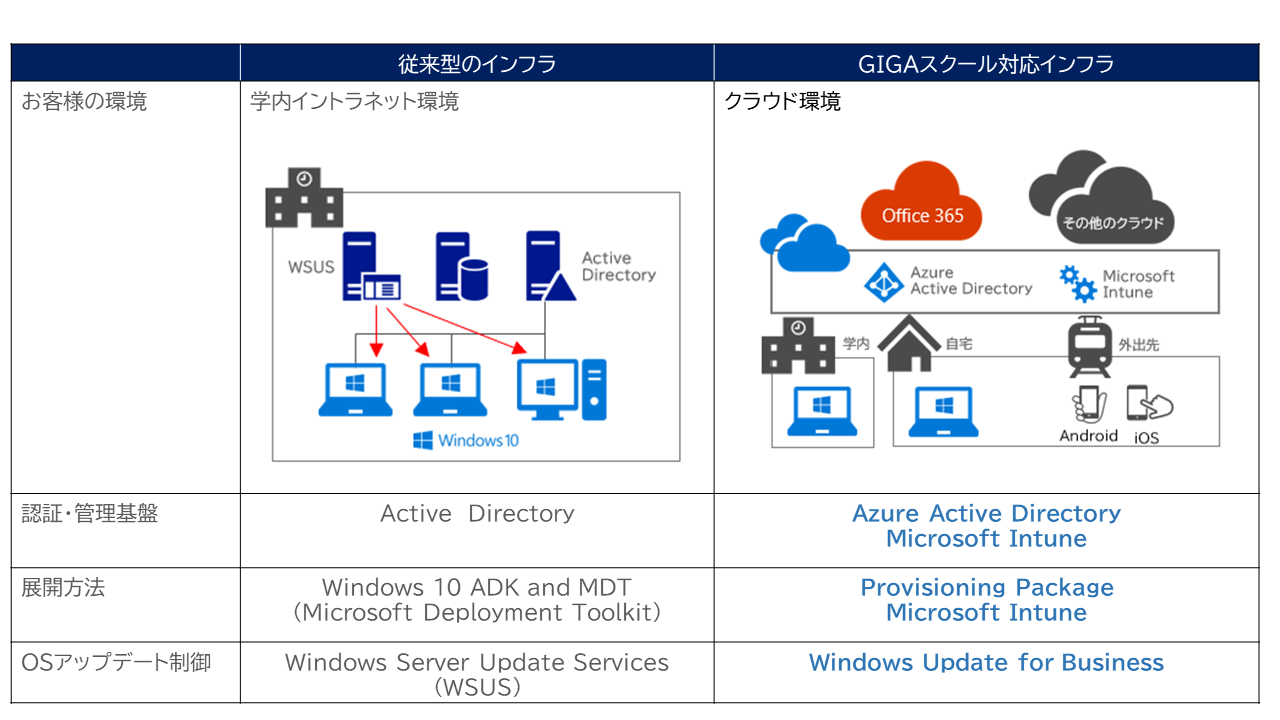
\includegraphics[width=16cm]{figures/Infrastructure.png}
    \caption{従来型のインフラストラクチャとGIGAスクール対応のインフラストラクチャの違い}
    \label{fig:Infra}
\end{figure*}

%%%%%%%%%%%%%%%%%%%%%%%%%%%%%%%%%%%%%%%%%%%%%%%%%%%%%%%%%%%%%%%%%%%%%%%%%%%%%%%%%
\section{Provisioning Package を利用したOOBE (Out of Box experience)}
\label{sec:ProvisioningPackage}
%%%%%%%%%%%%%%%%%%%%%%%%%%%%%%%%%%%%%%%%%%%%%%%%%%%%%%%%%%%%%%%%%%%%%%%%%%%%%%%%%

%%%%%%%%%%%%%%%%%%%%%%%%%%%%%%%%%%%%%%%%%%%%%%%%%%%%%%%%%%%%%%%%%%%%%%%%%%%%%%%%%
\subsection{Provisioning Package とは}
\label{ProvisioningPackageとは}
%%%%%%%%%%%%%%%%%%%%%%%%%%%%%%%%%%%%%%%%%%%%%%%%%%%%%%%%%%%%%%%%%%%%%%%%%%%%%%%%%

従来のディスクイメージによるクローニング展開は、PC購入時にプリインストールされているOSや各種アプリケーションを全て消去し、新規にOSや各種アプリケーションをインストールし直して作成したディスクイメージをもとに、複数のPCにクローニング展開を行う方法です。

一方、「Provisioning Package」 は、プリインストールされているOSやアプリケーションを利用し、その上で必要な設定だけを加えることで業務用PCとして利用可能にする手法です。プロビジョニングパッケージという ppkg ファイルが保存された USB メモリーを初回起動時の PC に挿入するだけで、ホスト名やアカウント作成をはじめとする初期設定が実施できます。\\

%%%%%%%%%%%%%%%%%%%%%%%%%%%%%%%%%%%%%%%%%%%%%%%%%%%%%%%%%%%%%%%%%%%%%%%%%%%%%%%%%
\subsection{Provisining Package でできること}
\label{sec:ProvisioningPackageできること}
%%%%%%%%%%%%%%%%%%%%%%%%%%%%%%%%%%%%%%%%%%%%%%%%%%%%%%%%%%%%%%%%%%%%%%%%%%%%%%%%%

Provisioning Package は、Windows 構成管理デザイナーという Windows ADK (アセスメント \& デプロイメントキット) に含まれるプログラムを使って作成します。 ウィザード形式、もしくは詳細エディターを使用して設定ます。ウィザード形式と詳細エディターでそれぞれ設定できる項目が異なります。「GIGAスクールパッケージ」では、Provisioning Package では最低限の設定し行いませんので、ここではウィザード形式での設定項目に関して説明します。

 以下に Windows 構成デザイナーのウィザード形式でプロビジョニングパッケージを作成する際に、設定できる項目について記載します。

\begin{description}
    \item[デバイス名]\mbox{}\\
        デバイス名は一意な15文字の名前を入力してください。一意な名前を生成する方法としては、「\tt{\%SERIAL\%}」を使ってハードウェア固有のシリアル番号を名前に含めるか、「\tt{\%RAND:x\%}」を使って長さ x のランダムな文字を生成することができます。\\
        デバイス名の例\\
         \tt{Contoso-\%SERIAL\%}\\
         \tt{Fabrikan-\%RANDAN:5\%}
    \item[プロダクトキー]\mbox{}\\
        プロダクトキーを入力して、Windowsをアップグレードすることができます。エディションを変更したい場合に設定することができます。
    \item[共有するためのデバイス構成]\mbox{}\\
        このオプションをYes(はい)にすると複数のユーザーでデバイスを共有することができるようになります。
    \item[プレインストールされているソフトウェアの削除]\mbox{}\\
        ユーザーデータを保存せず、プレインストールされているソフトウェアを削除することができます。ただし、必要なドライバー、ユーティリティーまで削除されてしまうことがありますので、注意が必要です。このオプションをYes(はい)にするとキッティング作業に時間がかかりますので、通常はNo(いいえ)にしてください。
    \item[Wi-Fi(SSID)]\mbox{}\\
        Wi-Fiに接続するためのSSID、パスワードを設定することができます。Wi-Fiの認証方式は、Open(パスワードなし)か、WPA2-Personal の2つのみとなっています。
    \item[アカウントの管理]\mbox{}\\
        デバイスを Active Directory へ登録したり、Azure Active Directory に登録することができます。またローカル管理者を作成することもできます。
    \item[アプリケーションのインストール]\mbox{}\\
        サイレントインストールに対応したアプリケーションを追加することができます。コマンドライン引数を設定できるので、例えば、「\tt{¥cmd \/c “lpls174.exe” \/silent \/norestart}」 といった形で設定しておくことで、プロビジョニングパッケージを実行した時にアプリケーションがサイレントインストールされます。MSI形式でも問題ありません。ただし Provisioning Package でインストールしたパッケージは Intune では管理できませんので、今回は何もインストールしません。
    \item[証明書の追加]\mbox{}\\
        デバイスに任意の証明書を追加することができます。デバイス認証等で証明書を追加する場合に設定します。
\end{description}

プロビジョニングパッケージを使用する上での注意点を記載します。以下の注意点をお読みいただき、問題ないと判断できればプロビジョニングパッケージによるOS展開が可能だと考えていただければと思います。

\begin{enumerate}
    \renewcommand{\labelenumi}{\alph{enumi})}
    \item 更新機能プログラム毎にパッケージ製作が必要
    \item アプリケーションの追加には、サイレントインストールに対応が必須
    \item アプリケーションの追加は、何かしらの理由で失敗する可能性がある
    \item アプリケーションの設定は変更できない(インストールのみ)
    \item プロビジョニングパッケージの実行は30秒以内に終える必要がある
    \item ホスト名はプレフィックスを除き、製造番号かランダム値しか選べない
    \item ユーザー情報を消す場合は、プレインストールされているソフトウェアも削除される
\end{enumerate}

%%%%%%%%%%%%%%%%%%%%%%%%%%%%%%%%%%%%%%%%%%%%%%%%%%%%%%%%%%%%%%%%%%%%%%%%%%%%%%%%%
\subsection{Windows 構成デザイナーのインストール}
\label{sec:Windows構成デザイナーのインストール}
%%%%%%%%%%%%%%%%%%%%%%%%%%%%%%%%%%%%%%%%%%%%%%%%%%%%%%%%%%%%%%%%%%%%%%%%%%%%%%%%%

Provisioning Package を作成するためにはWindows構成デザイナー(Windows Configuration Designer)が必要です。Windows 構成デザイナーは、Windows 10 を実行しているデバイスでは、 Microsfot Stora から Windows Configuration Designer アプリをインストールすることができます。
他のオペレーティングシステムまたは英語以外の言語でWindows構成デザイナーを実行したい場合には、Windows 10 用 Windows アセスメント \& ディプロイメントキット (ADK)\footnote{\url{https://docs.microsoft.com/ja-jp/windows-hardware/get-started/adk-install}}をインストールしてください。

\begin{figure}[htbp]
    \centering
    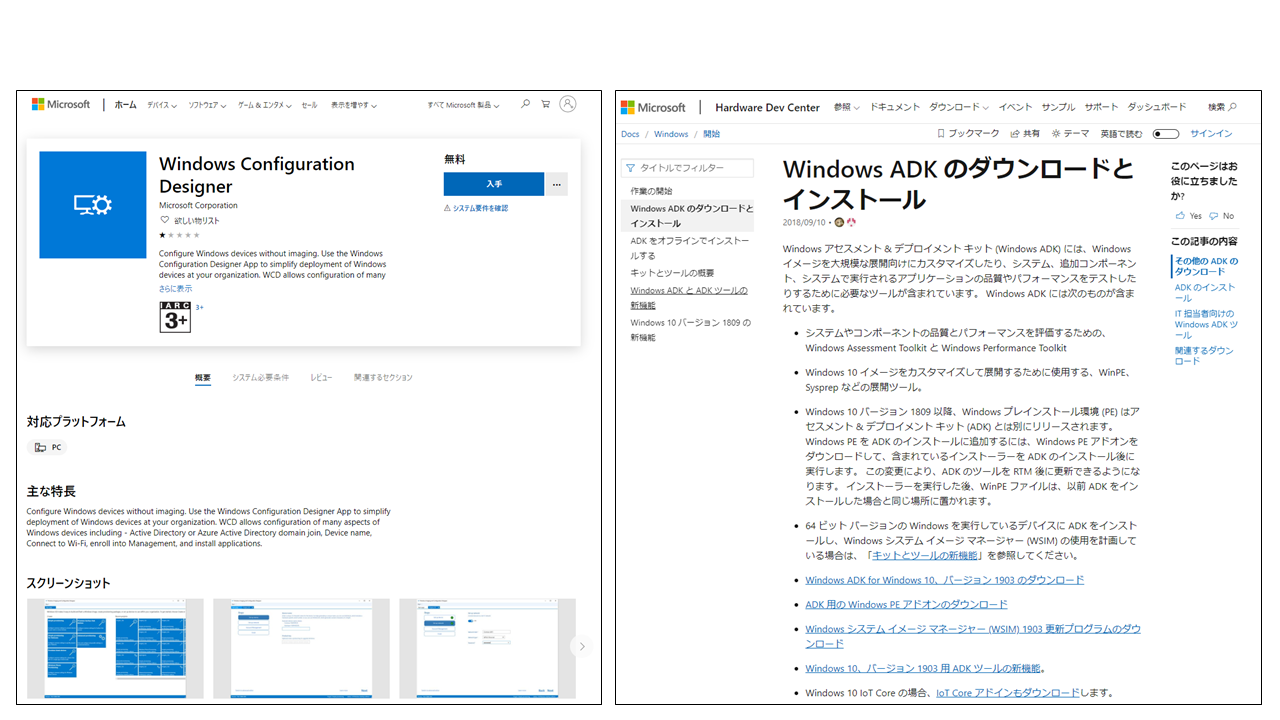
\includegraphics[width=17cm]{figures/WindowsConfigurationDesigner.png}
    \caption{Windows構成デザイナーのインストール}
    \label{fig:WindowsConfigutionDesigner}
    \vspace{6cm}
\end{figure}

%%%%%%%%%%%%%%%%%%%%%%%%%%%%%%%%%%%%%%%%%%%%%%%%%%%%%%%%%%%%%%%%%%%%%%%%%%%%%%%%%
\begin{figure}[htbp]
    \subsection{Microsoft Store版 Windows Configuration Designer のインストール}
\end{figure}
%%%%%%%%%%%%%%%%%%%%%%%%%%%%%%%%%%%%%%%%%%%%%%%%%%%%%%%%%%%%%%%%%%%%%%%%%%%%%%%%%

\begin{figure*}[hp]
    \begin{minipage}{0.6\textwidth}
        \vspace{0cm}
        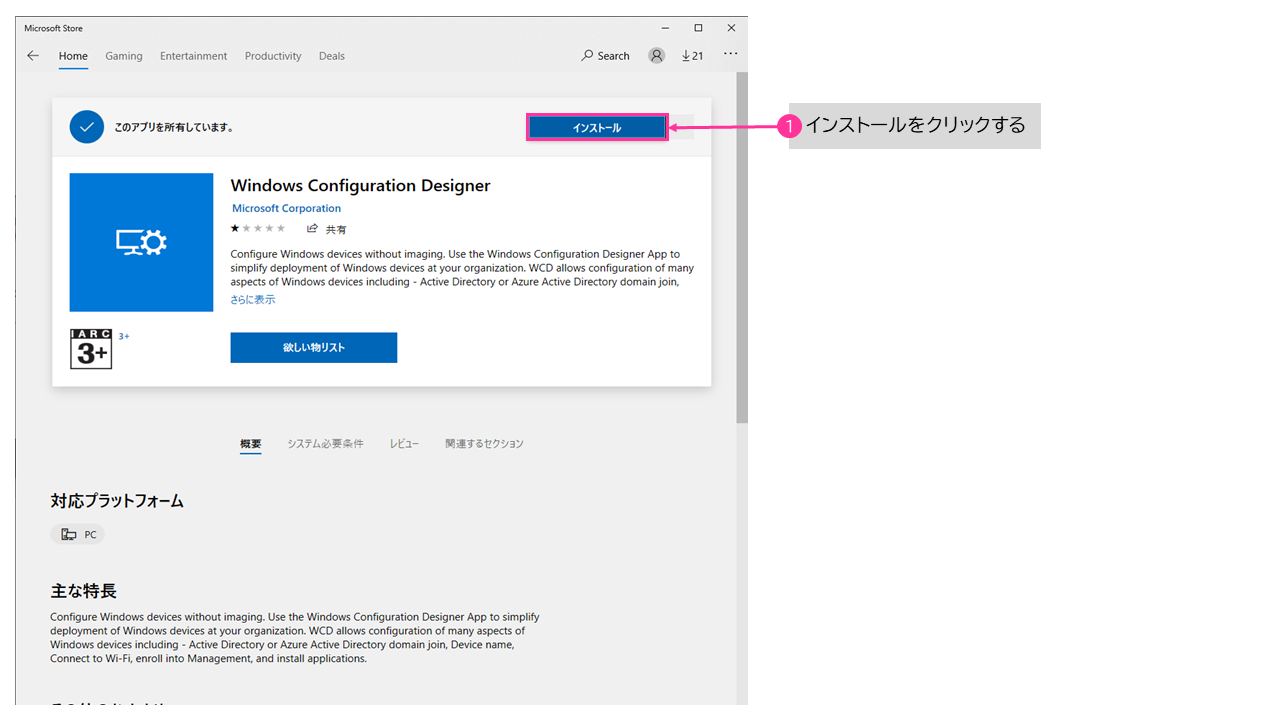
\includegraphics[width=10cm]{figures/Install_WinConfDisgn.png}
    \end{minipage}
    \begin{minipage}{0.4\textwidth}
        Microsoft Store にアクセスして、検索バーでWindows Configuration Designer と入力します。Windows Configuration Designer の画面が表示されましたら\textbf{【インストール】}ボタンをクリックしてください。
    \end{minipage}
    \vspace{3cm}
\end{figure*}

%%%%%%%%%%%%%%%%%%%%%%%%%%%%%%%%%%%%%%%%%%%%%%%%%%%%%%%%%%%%%%%%%%%%%%%%%%%%%%%%%
\begin{figure}[htbp]
    \subsection{Windows アセスメント \& ディプロイメントキット (ADK) のインストール}
\end{figure}
%%%%%%%%%%%%%%%%%%%%%%%%%%%%%%%%%%%%%%%%%%%%%%%%%%%%%%%%%%%%%%%%%%%%%%%%%%%%%%%%%

\begin{figure*}[h]
    \begin{minipage}{0.6\textwidth}
        \vspace{0cm}
        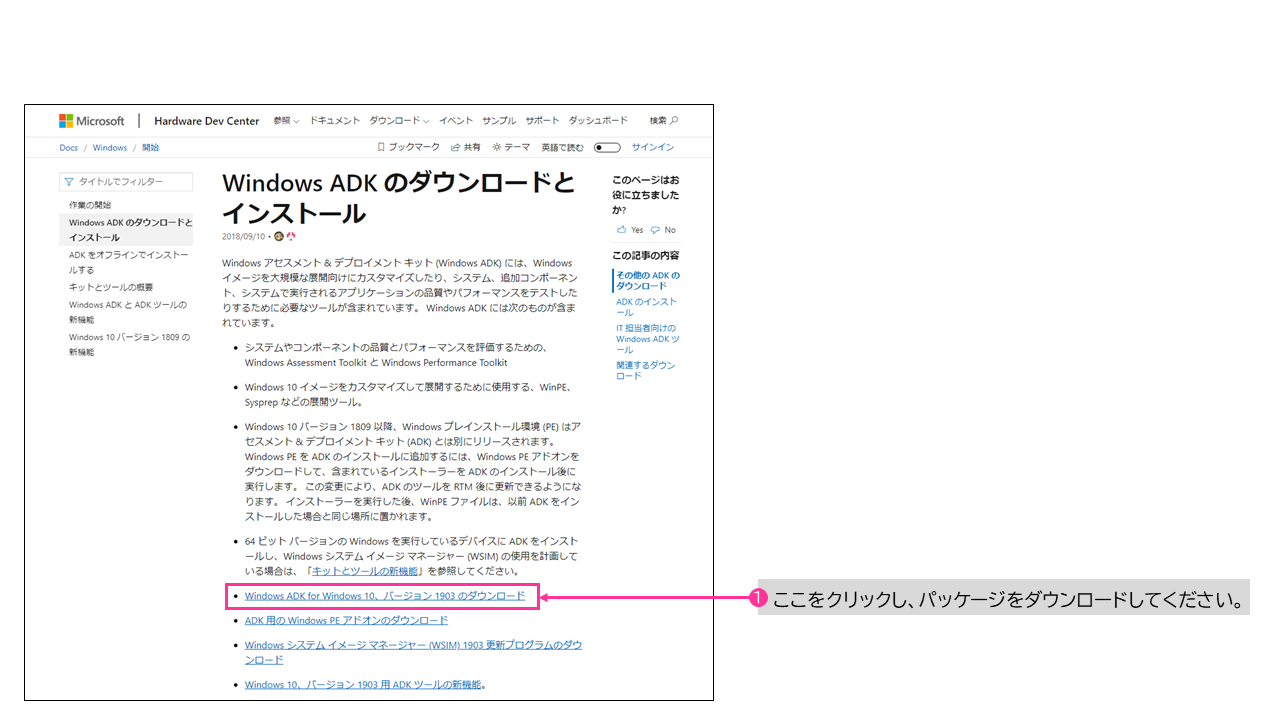
\includegraphics[width=10cm]{figures/Install_WinADK-01.png}
    \end{minipage}
    \begin{minipage}{0.4\textwidth}
        Webブラウザで Windows ADK のダウンロードページ\protect\footnotemark
        から該当するバージョンのASK(\tt{adksetup.exe})をダウンロードしてください。
    \end{minipage}
\end{figure*}
\footnotetext{\url{https://docs.microsoft.com/ja-jp/windows-hardware/get-started/adk-install}}

\begin{figure*}[hp]
    \begin{minipage}{0.6\textwidth}
        \vspace{0cm}
        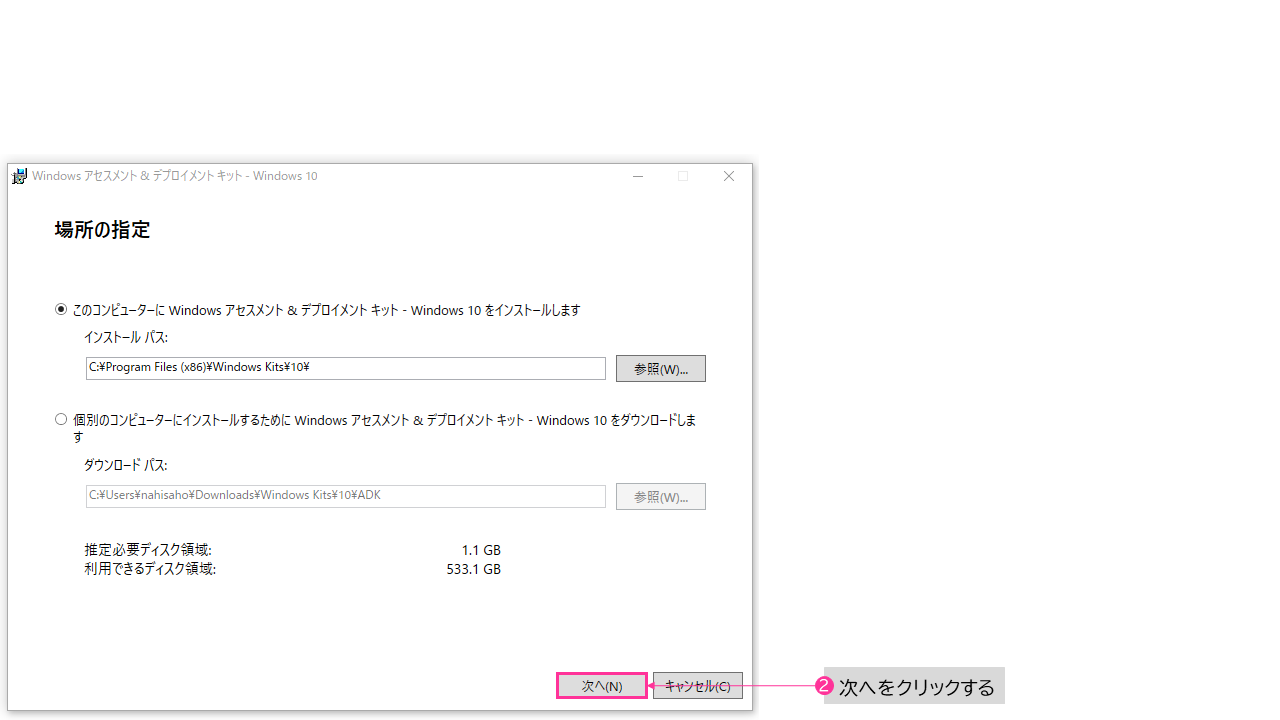
\includegraphics[width=10cm]{figures/Install_WinADK-02.png}
    \end{minipage}
    \begin{minipage}{0.4\textwidth}
        ダウンロードしたtt{adksetup.exe}を管理者権限でダブルクリックします。
    \end{minipage}
\end{figure*}

\begin{figure*}[hp]
    \begin{minipage}{0.6\textwidth}
        \vspace{0cm}
        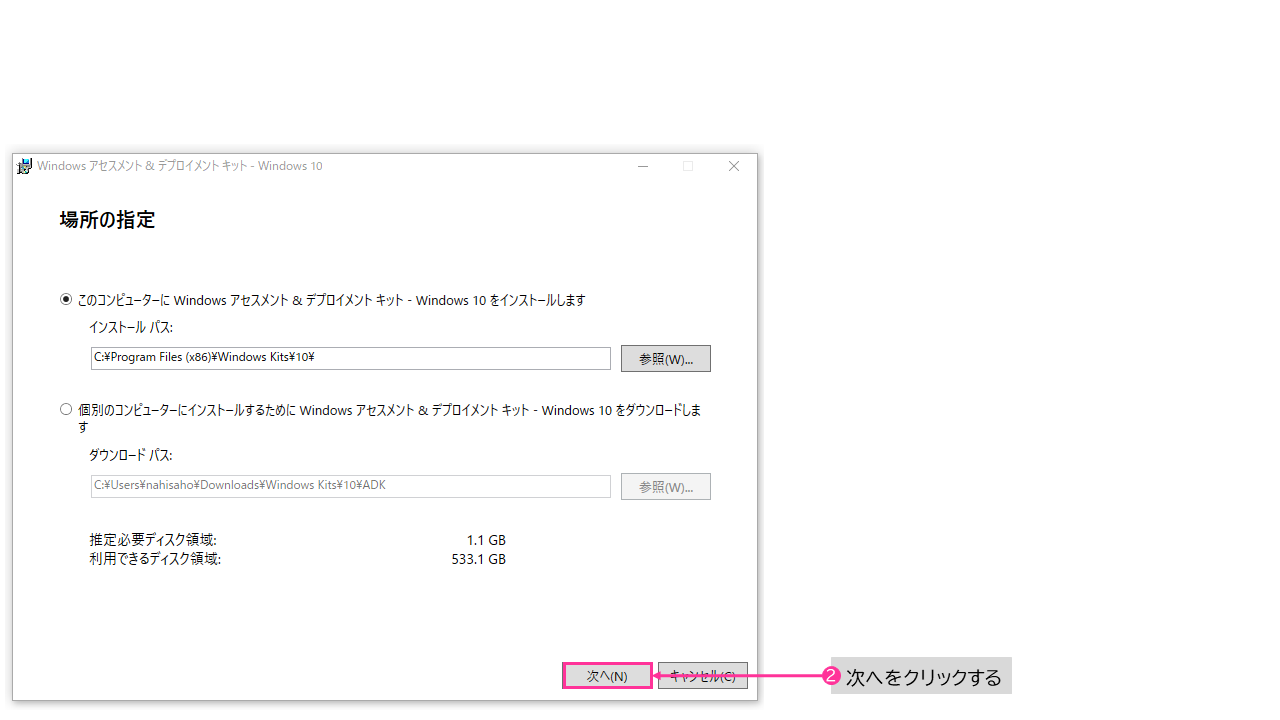
\includegraphics[width=10cm]{figures/Install_WinADK-03.png}
    \end{minipage}
    \begin{minipage}{0.4\textwidth}
        \textbf{「場所を指定」}の画面が表示されたら、\textbf{【次へ(N)】}をクリックしてください。
    \end{minipage}
\end{figure*}

\begin{figure*}[hp]
    \begin{minipage}{0.6\textwidth}
        \vspace{0cm}
        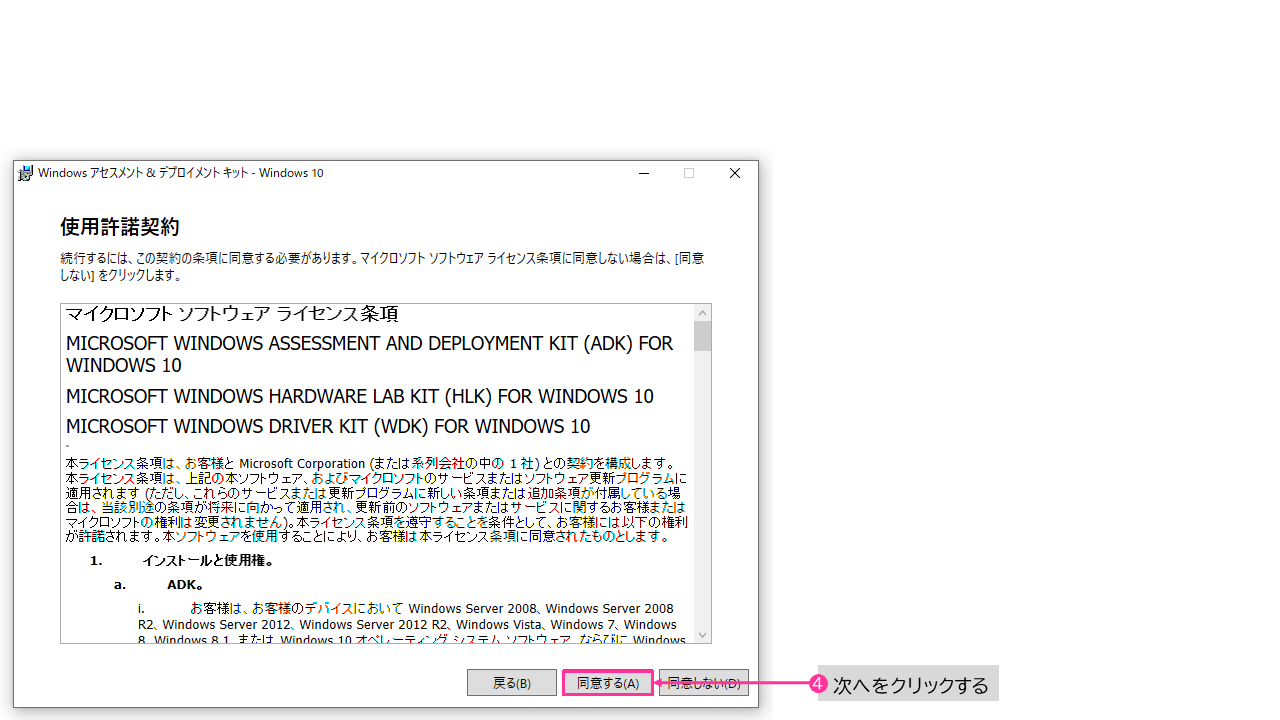
\includegraphics[width=10cm]{figures/Install_WinADK-04.png}
    \end{minipage}
    \begin{minipage}{0.4\textwidth}
        \textbf{「使用許諾契約」}の画面が表示ます。内容を確認し、\textbf{【同意する(A))】}をクリックしてください。
    \end{minipage}
\end{figure*}

\begin{figure*}[hp]
    \begin{minipage}{0.6\textwidth}
        \vspace{-0.5cm}
        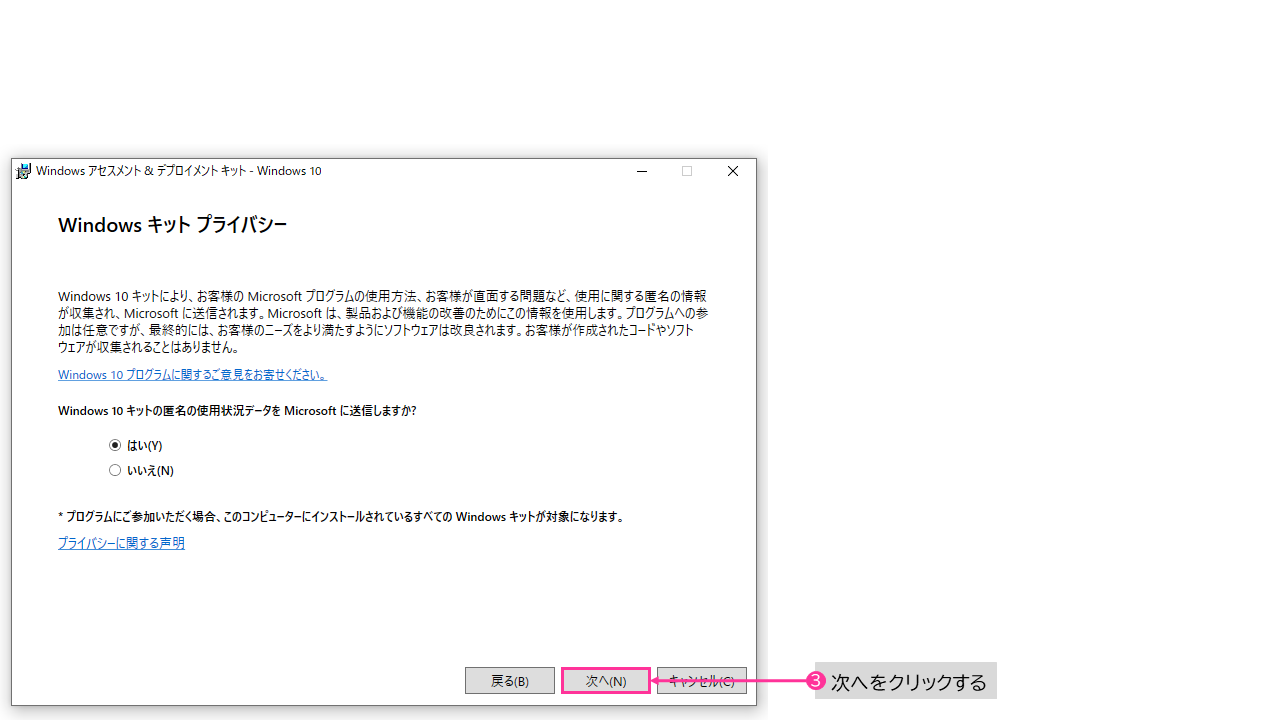
\includegraphics[width=10cm]{figures/Install_WinADK-05.png}
    \end{minipage}
    \begin{minipage}{0.4\textwidth}
        \textbf{「Windowsキットプライバシー」}の画面が表示ます。Windows 10キットの匿名の使用状況データをMicrosoftに送信して問題ないようであれば、\textbf{【はい】}を、そうでない場合は\textbf{【いいえ】}を選択して、\textbf{【次へ(N)】}をクリックしてください。
    \end{minipage}
\end{figure*}

\begin{figure*}[hp]
    \begin{minipage}{0.6\textwidth}
        \vspace{0cm}
        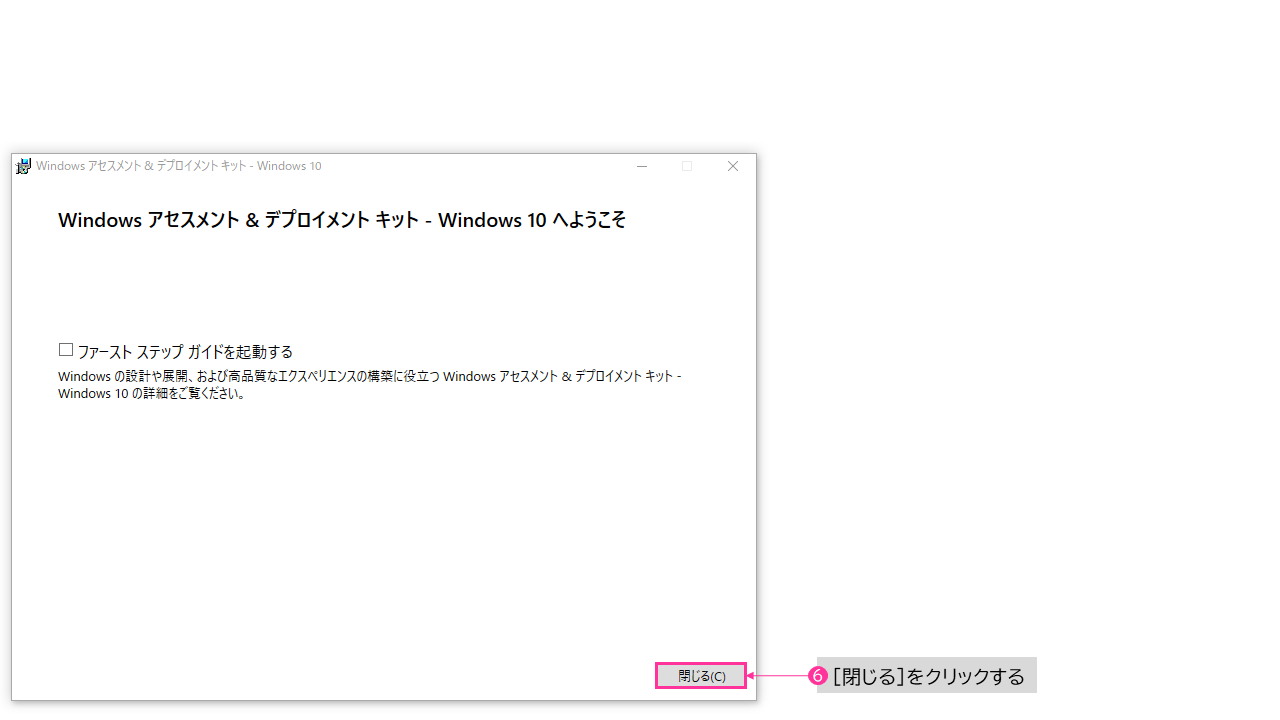
\includegraphics[width=10cm]{figures/Install_WinADK-07.png}
    \end{minipage}
    \begin{minipage}{0.4\textwidth}
        インストールが完了しましたら、\textbf{【閉じる(C)】}をクリックしてください。
    \end{minipage}
    \vspace{3cm}
\end{figure*}

\newpage

%%%%%%%%%%%%%%%%%%%%%%%%%%%%%%%%%%%%%%%%%%%%%%%%%%%%%%%%%%%%%%%%%%%%%%%%%%%%%%%%%
\begin{figure}[htbp]
    \subsection{Provisioning Package の作成}
    \label{sec:ProvisioningPackageの作成}

    \hspace{8pt} \ref{sec:ProvisioningPackageの作成}項では、Windows 構成デザイナーを使用して Provisioning Package を作成する方法に関して解説いたします。
\end{figure}
%%%%%%%%%%%%%%%%%%%%%%%%%%%%%%%%%%%%%%%%%%%%%%%%%%%%%%%%%%%%%%%%%%%%%%%%%%%%%%%%%

\begin{figure*}[hp]
    \begin{minipage}{0.6\textwidth}
        \vspace{-1.5cm}
        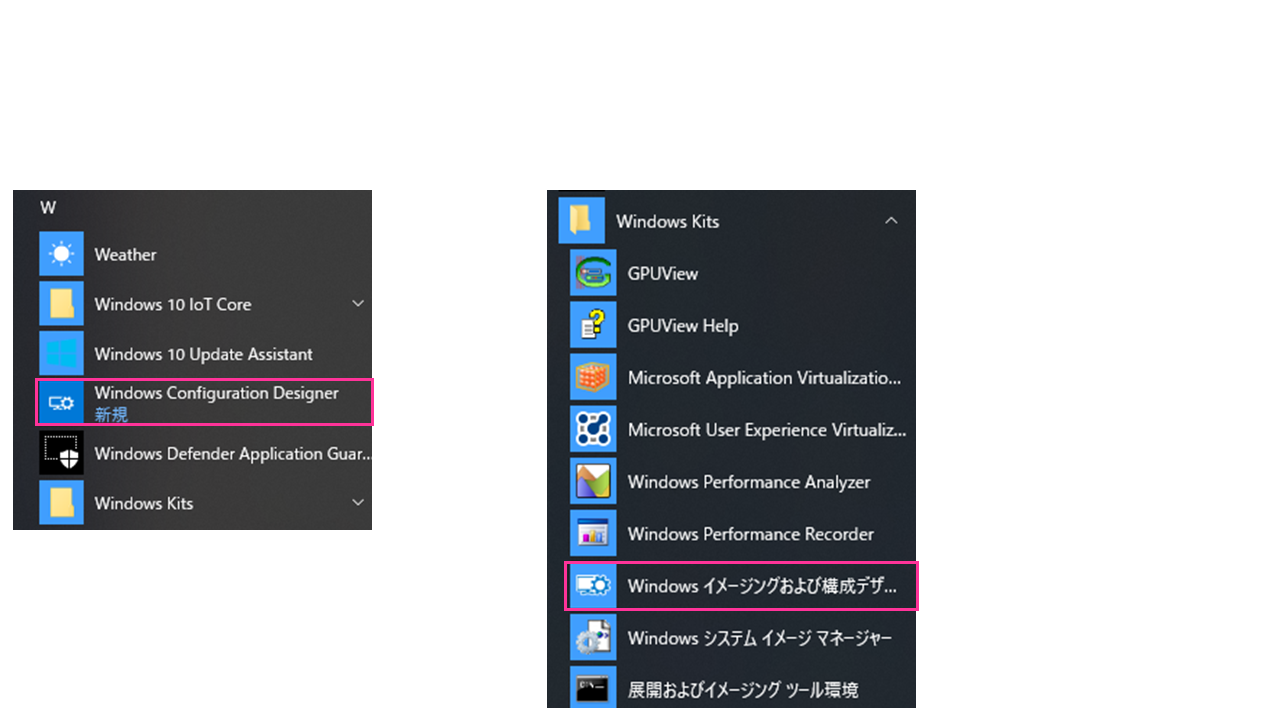
\includegraphics[width=10cm]{figures/MakeProvisioningPackage-01}
    \end{minipage}
    \begin{minipage}{0.4\textwidth}
        Windows 構成デザイナーを起動します。Microsoft Store 版をインストールされた方は、\textbf{Windows Configuration Designer}を、Windows ADK をインストールされた方は、Windows Kits の下の\textbf{WIndowsイメージングおよび構成デザイナー}をクリックして、Windows構成デザイナーを起動してください。
    \end{minipage}
\end{figure*}

\begin{figure*}[hp]
    \begin{minipage}{0.6\textwidth}
        \vspace{0cm}
        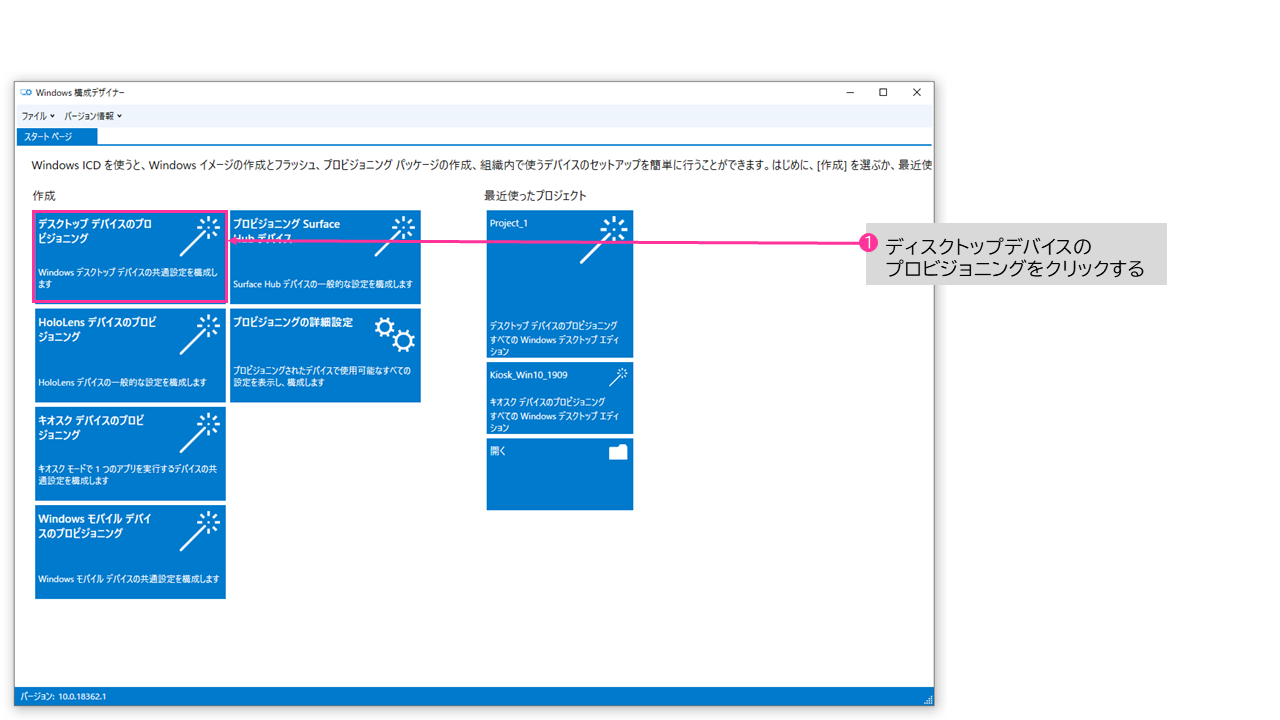
\includegraphics[width=10cm]{figures/MakeProvisioningPackage-02}
    \end{minipage}
    \begin{minipage}{0.4\textwidth}
        Windows 構成デザイナーが起動したら、\textbf{【デスクトップデバイスのプロビジョニング}をクリックします。
    \end{minipage}
\end{figure*}


\begin{figure*}[hp]
    \begin{minipage}{0.6\textwidth}
        \vspace{-2.5cm}
        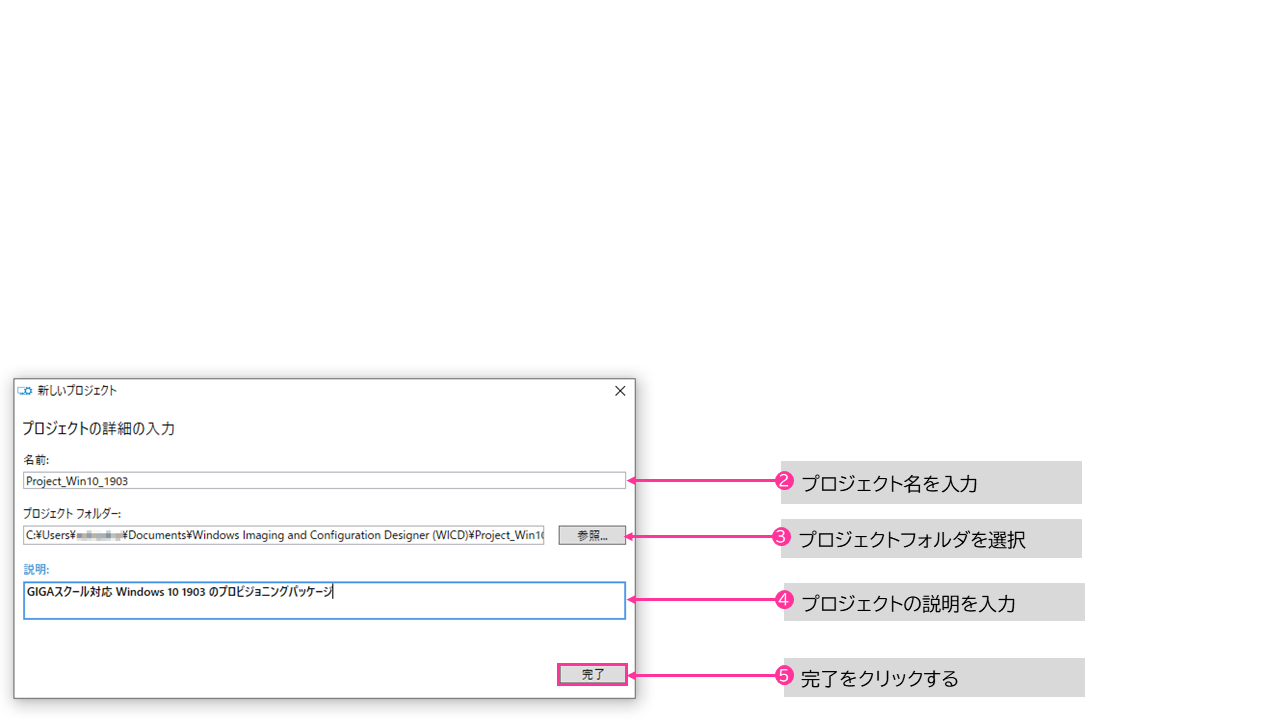
\includegraphics[width=9cm]{figures/MakeProvisioningPackage-03}
    \end{minipage}
    \begin{minipage}{0.4\textwidth}
        \textbf{「新しいプロジェクト」}の画面が開いたら、プロジェクト名、プロジェクトフォルダー、プロジェクトの説明を入力し、\textbf{【完了】}をクリックしてください。
    \end{minipage}
\end{figure*}

\begin{figure*}[hp]
    \begin{minipage}{0.6\textwidth}
        \vspace{-0.5cm}
        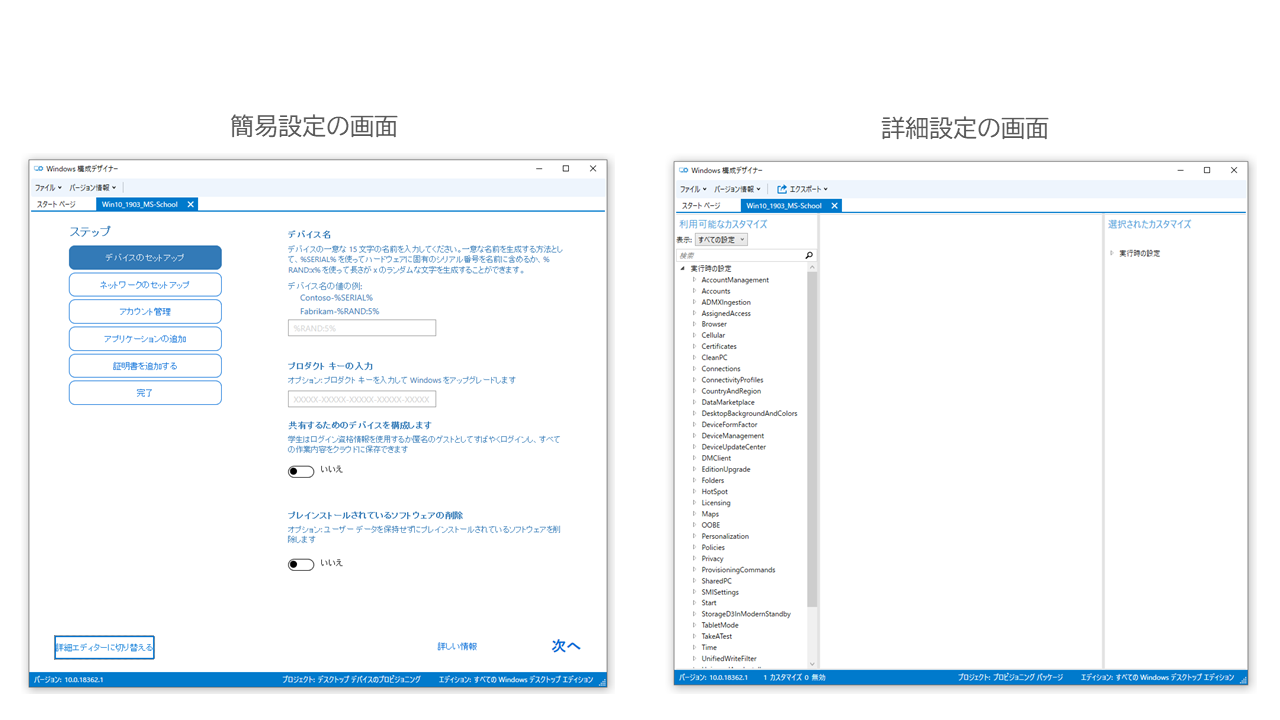
\includegraphics[width=10cm]{figures/MakeProvisioningPackage-04}
    \end{minipage}
    \begin{minipage}{0.4\textwidth}
        Windows構成デザイナーには、\text{簡易設定(デフォルト)}と\textbf{詳細設定}の2種類のモードが用意されています。詳細設定を行いたい場合は、画面左下の\textbf{【詳細エディターに切り替える】}をクリックしてください。\textbf{GIGAスクールで設定しなければいけない項目は、簡易設定で全て行えますので、この後の解説は簡易設定に限定致します。}
    \end{minipage}
\end{figure*}

\begin{figure*}[hp]
    \begin{minipage}{0.6\textwidth}
        \vspace{-2.5cm}
        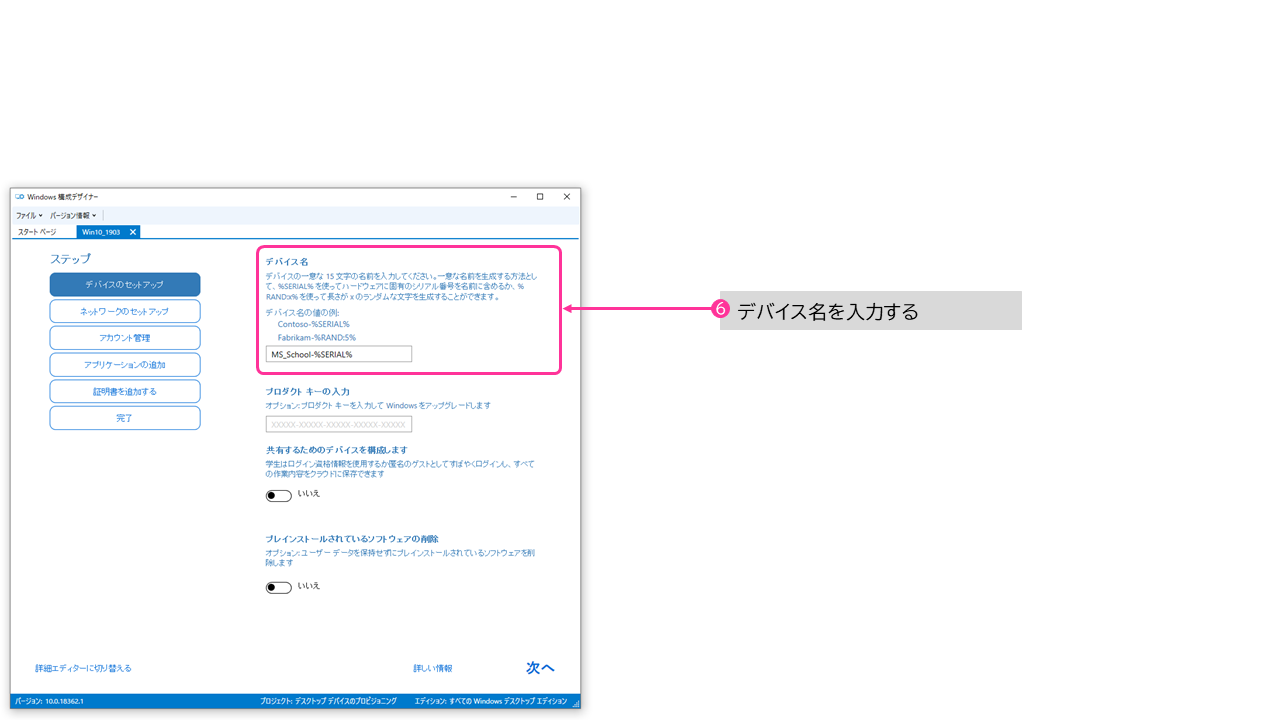
\includegraphics[width=10cm]{figures/MakeProvisioningPackage-05}
    \end{minipage}
    \begin{minipage}{0.4\textwidth}
        \textbf{「デバイスのセットアップ」}では、まずはじめにデバイス名を入力します。デバイス名はテナント内で一意である必要があります。デバイス名を一意にする方法としては 
        \begin{enumerate}
            \item ハードウェア固有のシリアル番号を利用する方法
            \item indows構成デザイナーでランダムな文字列を自動生成する方法
        \end{enumerate}
        の2つの方法があります。

        GIGAスクール構想では、複数年度にわたり端末の調達がらいますので、1番のハードウェア固有のシリアル番号を利用する方法を選択してください。
    \end{minipage}
\end{figure*}

\begin{figure*}[hp]
    \begin{minipage}{0.6\textwidth}
        \vspace{-1cm}
        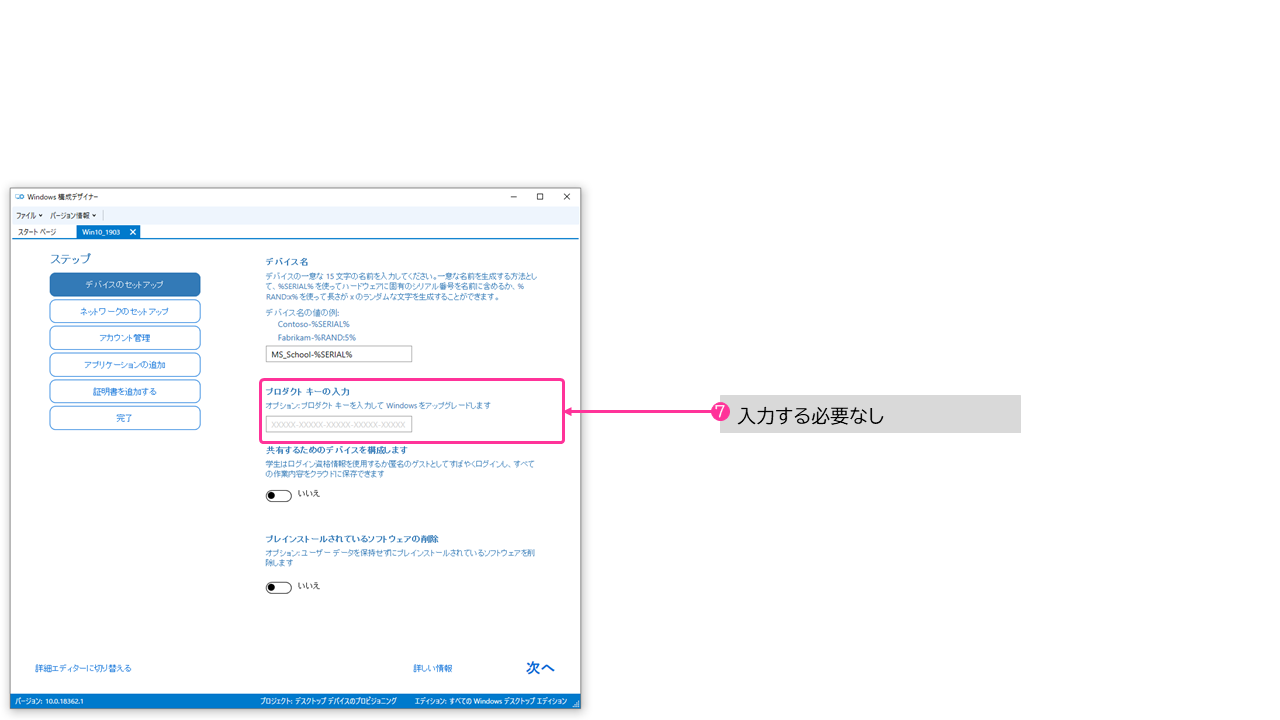
\includegraphics[width=10cm]{figures/MakeProvisioningPackage-06}
    \end{minipage}
    \begin{minipage}{0.4\textwidth}
        GIGAスクール対応のWindows PCには、Windows 10 Pro Education が標準てインストールされています。従って、Windows 10 をアップグレードする必要はございませんので、プロダクトキーを入力する必要はございません。
    \end{minipage}
\end{figure*}

\begin{figure*}[hp]
    \begin{minipage}{0.6\textwidth}
        \vspace{-1cm}
        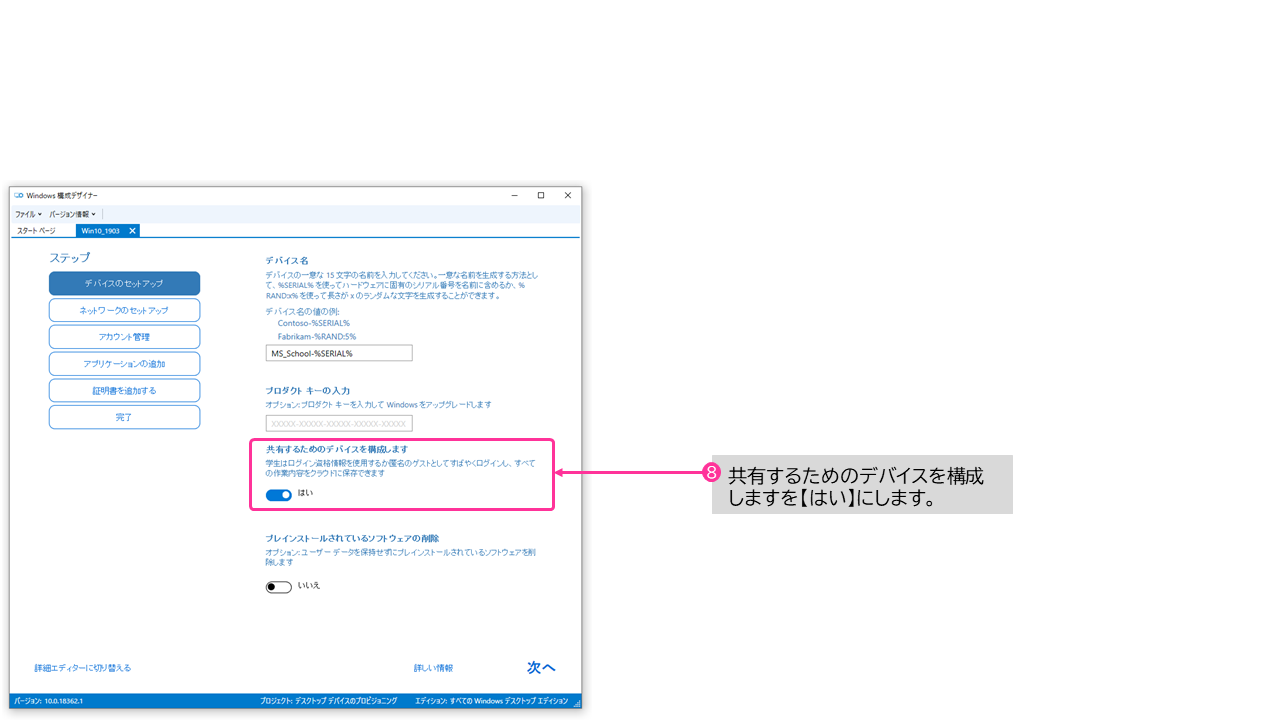
\includegraphics[width=10cm]{figures/MakeProvisioningPackage-07}
    \end{minipage}
    \begin{minipage}{0.4\textwidth}
        共有するためのデバイスを構成するを\textbf{【はい】}にします。これによりディスクの空き容量が足りなくなったりすると自動的にプロファイルを削除するようになり、ディスクの空き容量不足でWindows OSのアップデートに失敗することを防ぐことができます。
    \end{minipage}
\end{figure*}

\begin{figure*}[hp]
    \begin{minipage}{0.6\textwidth}
        \vspace{-1cm}
        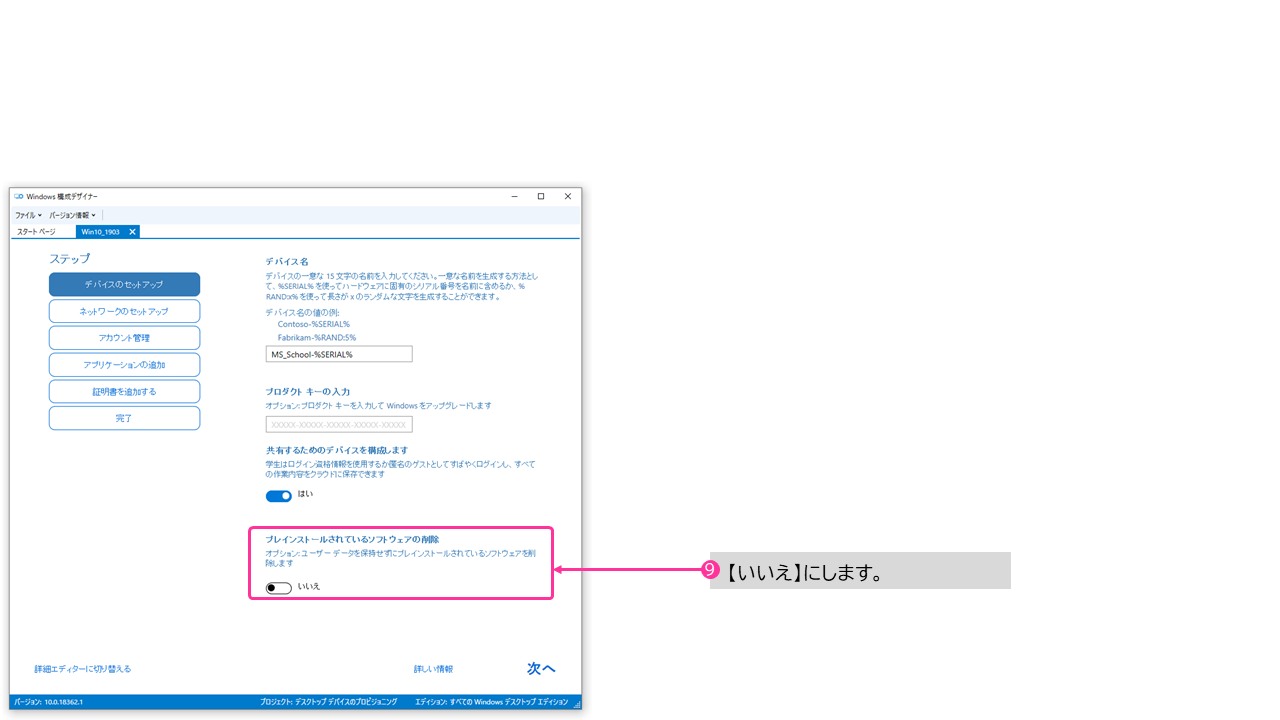
\includegraphics[width=10cm]{figures/MakeProvisioningPackage-08}
    \end{minipage}
    \begin{minipage}{0.4\textwidth}
        プレインストールされているソフトウェアを削除する場合には、\textbf{【はい】}にしてください。「はい」にした場合、Provisioning Package によるディプロイを実施する前に、端末を工場出荷時の状態に戻します。

        この作業に20~30分かかりますので、通常は\textbf{【いいえ】}にしてください。他人が使用してた端末を初期化して新たに人に配布したい場合には「はい」にしてください。
    \end{minipage}
\end{figure*}

\begin{figure*}[hp]
    \begin{minipage}{0.6\textwidth}
        \vspace{-1cm}
        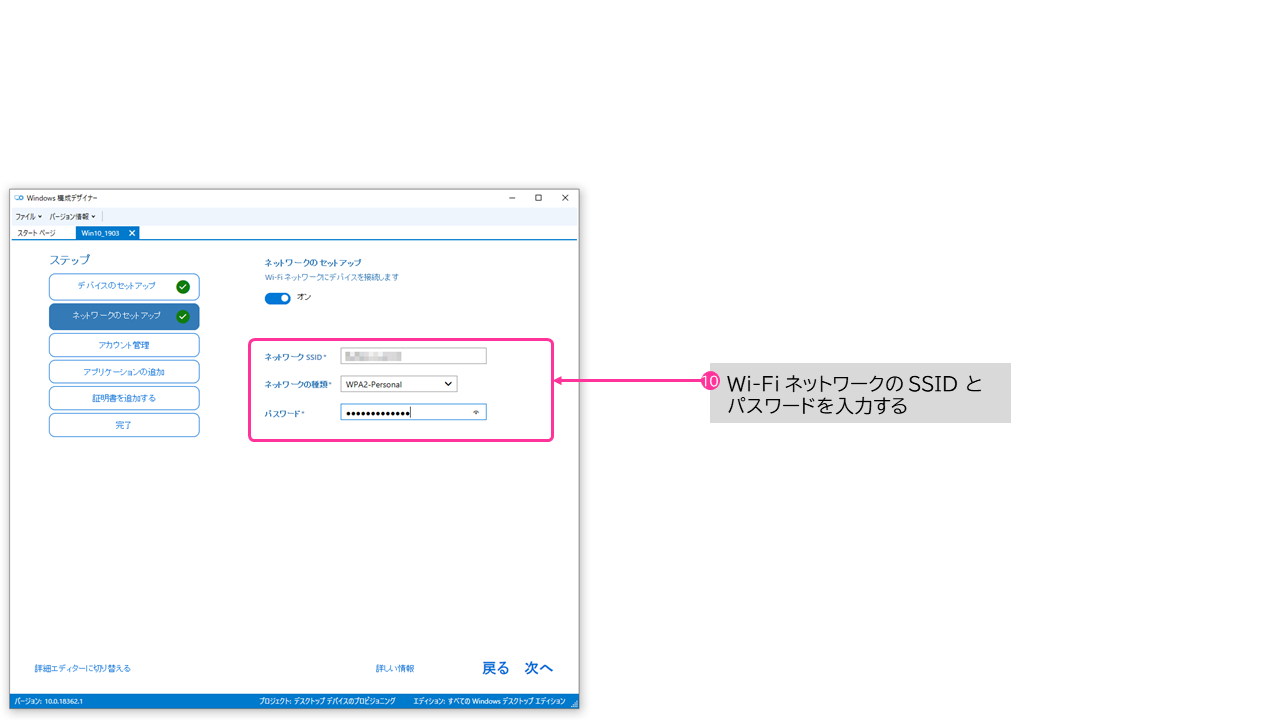
\includegraphics[width=10cm]{figures/MakeProvisioningPackage-09}
    \end{minipage}
    \begin{minipage}{0.4\textwidth}
        \textbf{「ネットワークのセットアップ」}では、Wi-Fiネットワークに接続するための設定が行えます。Provisioning Package では、Open もしくは WPA2-Personal に対応しています。ネットワークの設定が完了したら\textbf{【次へ】}をクリックしてください。
    \end{minipage}
\end{figure*}

\begin{figure*}[hp]
    \begin{minipage}{0.6\textwidth}
        \vspace{-1cm}
        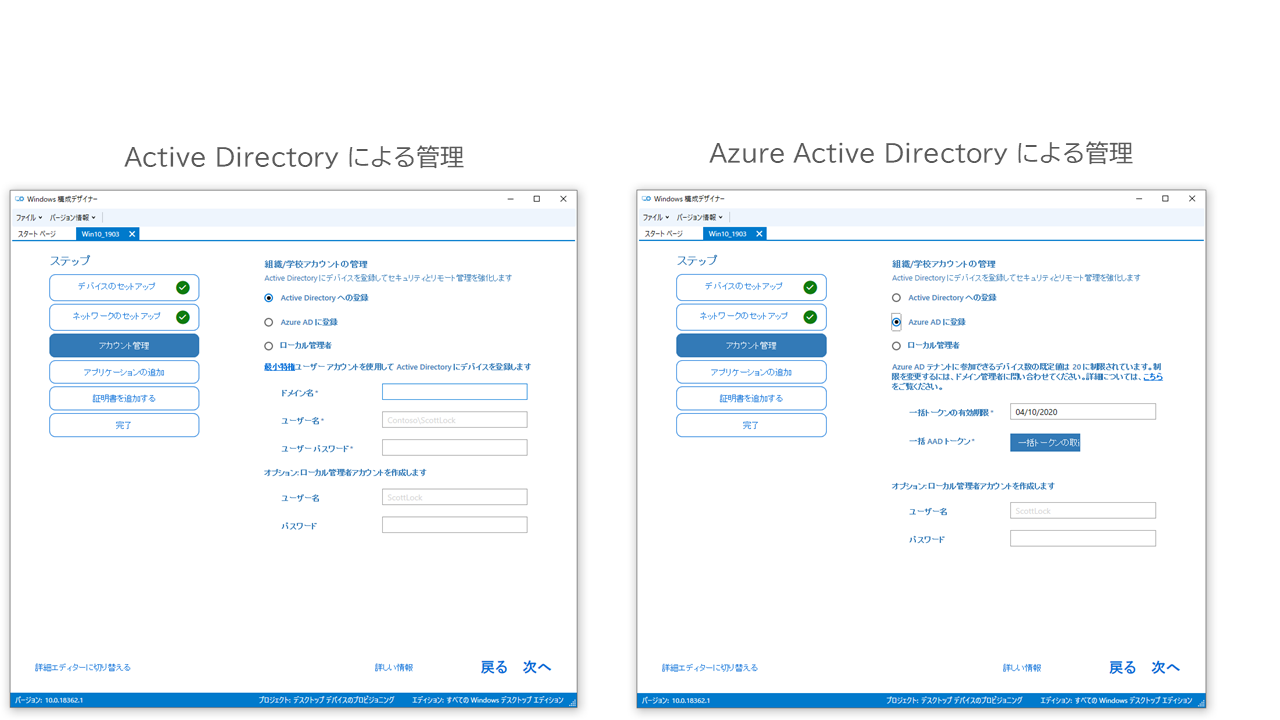
\includegraphics[width=10cm]{figures/MakeProvisioningPackage-10}
    \end{minipage}
    \begin{minipage}{0.4\textwidth}
        \textbf{「アカウント」}では、
        \begin{enumerate}
            \item Active Directory によるアカウント管理
            \item Azure Active DIrectory によるアカウント管理
            \item ローカルアカウントの作成
        \end{enumerate}
        が行えます。GIGAスクールパッケージでは、端末管理ツールに Intune for Education を利用しますので、2番目の Azure Active Directory によるアカウント管理を選択してください。
    \end{minipage}
\end{figure*}

\begin{figure*}[hp]
    \begin{minipage}{0.6\textwidth}
        \vspace{-1cm}
        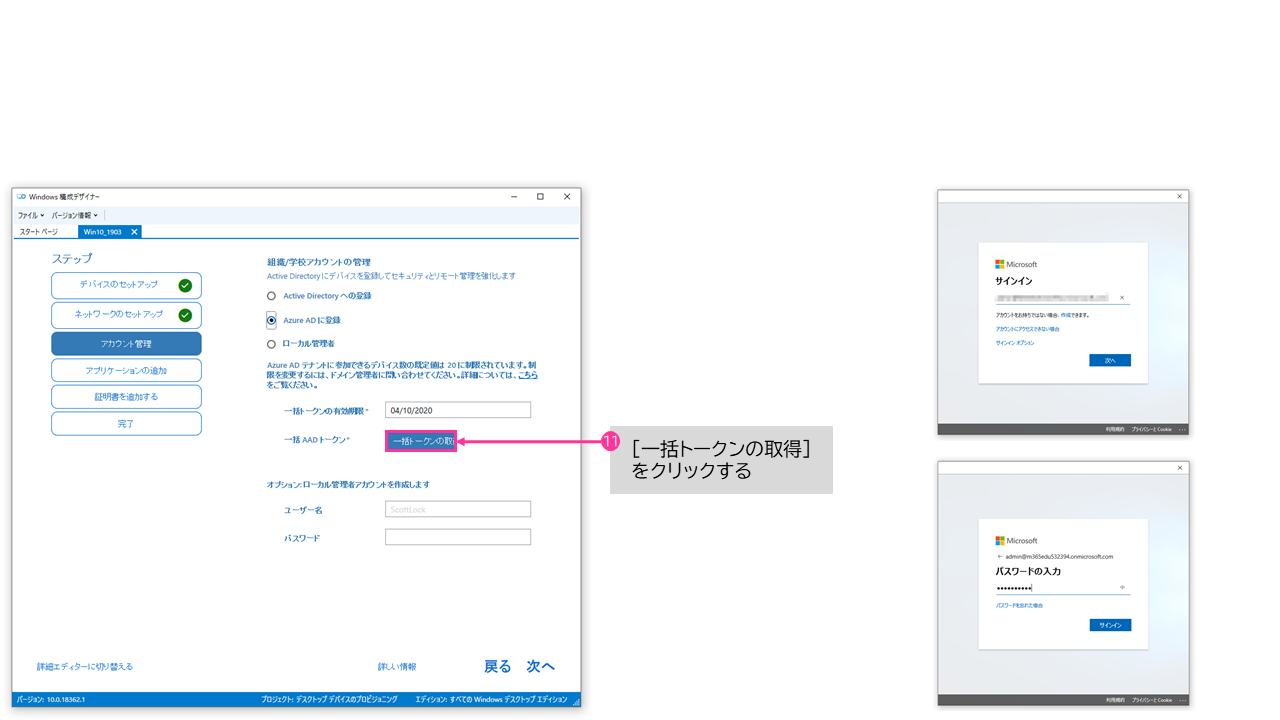
\includegraphics[width=10cm]{figures/MakeProvisioningPackage-11}
    \end{minipage}
    \begin{minipage}{0.4\textwidth}
        Azure Active Directory によるアカウント管理を行うには、\textbf{【Azure ADに登録します】}を選択します。一括トークンの有効期限を入力し、\textbf{【一括トークンの取得】}をクリックします。Office 365 の認証画面が表示されますので、管理者のアカウントとパスワードを入力してください。
    \end{minipage}
\end{figure*}

\begin{figure*}[hp]
    \begin{minipage}{0.6\textwidth}
        \vspace{-1cm}
        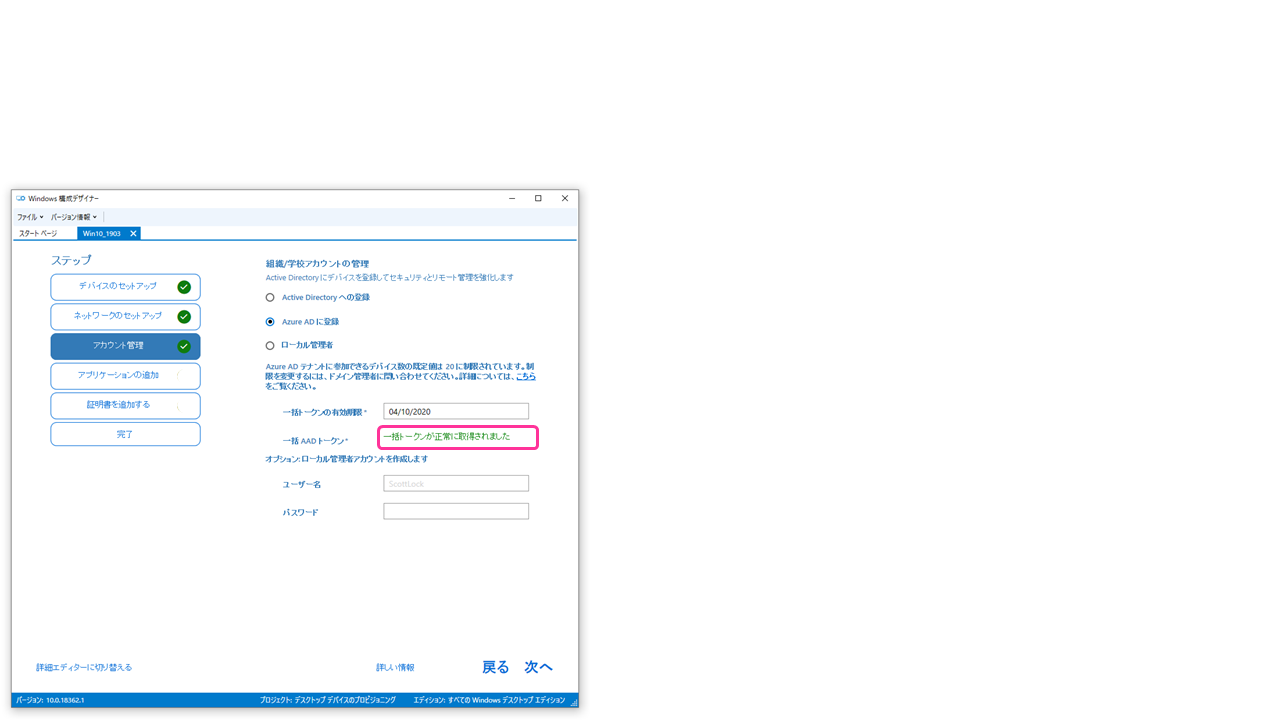
\includegraphics[width=10cm]{figures/MakeProvisioningPackage-12}
    \end{minipage}
    \begin{minipage}{0.4\textwidth}
        一括トークンの取得に成功すると、\textbf{【一括トークンが取得されました】}と表示されます。
    \end{minipage}
\end{figure*}

\begin{figure*}[hp]
    \begin{minipage}{0.6\textwidth}
        \vspace{-1cm}
        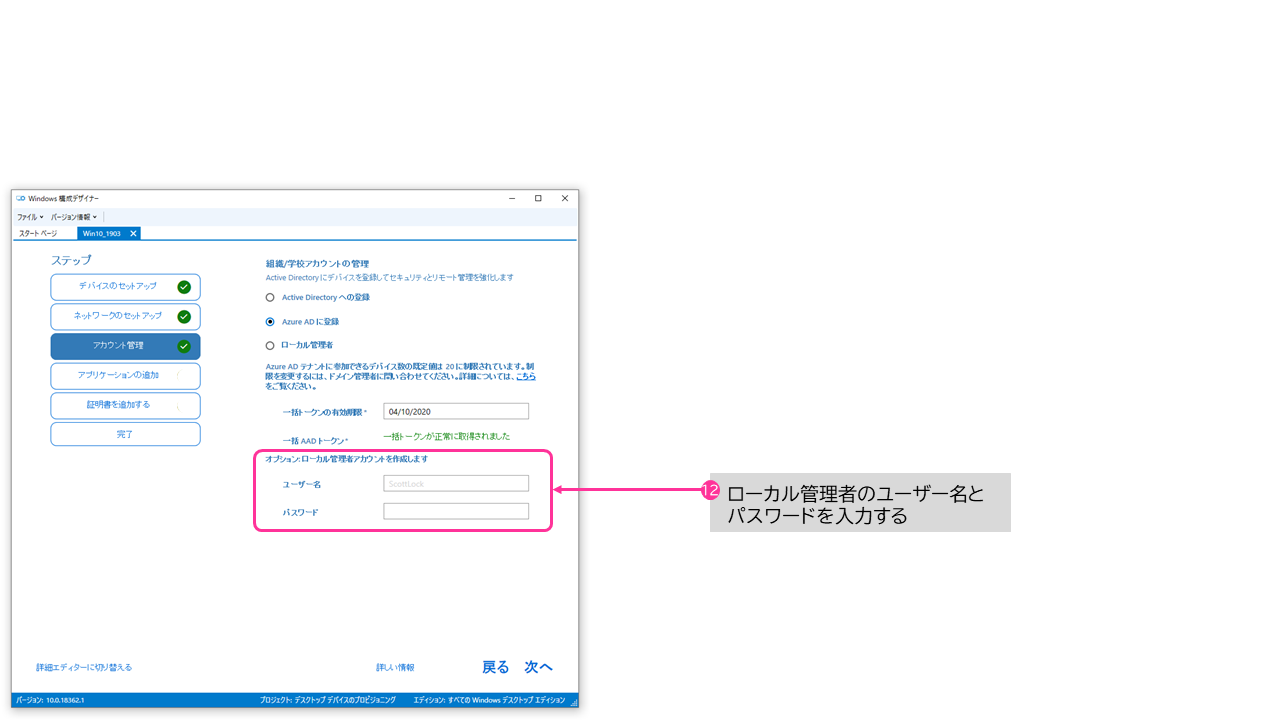
\includegraphics[width=10cm]{figures/MakeProvisioningPackage-13}
    \end{minipage}
    \begin{minipage}{0.4\textwidth}
        デバイス管理用にローカル管理者を作成したい場合には、ローカル管理者のユーザー名とパスワードを入力してください。
    \end{minipage}
\end{figure*}

\begin{figure*}[hp]
    \begin{minipage}{0.6\textwidth}
        \vspace{-1cm}
        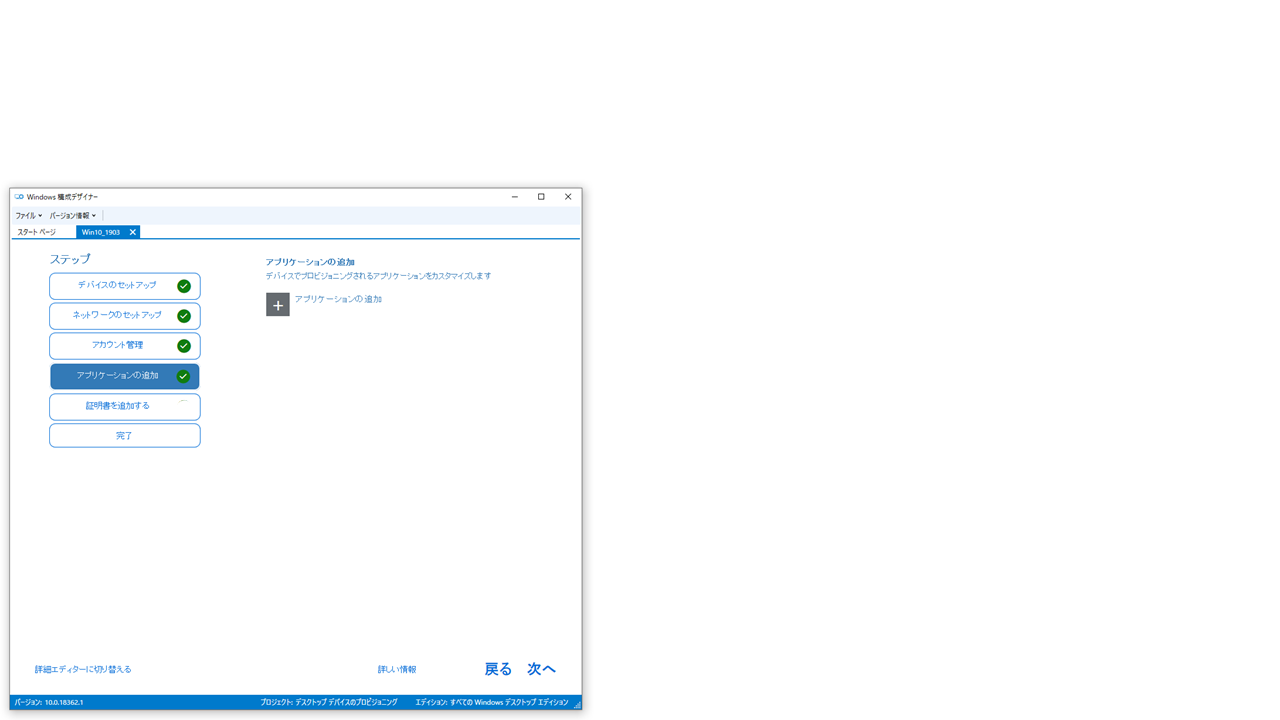
\includegraphics[width=10cm]{figures/MakeProvisioningPackage-14}
    \end{minipage}
    \begin{minipage}{0.4\textwidth}
        \textbf{「アプリケーションの追加」}では、アプリケーションの追加が行うことができます。ただし、Provisioning Package で追加したアプリケーションは端末管理ツール Intune では管理できなくなりますので、Provisioning Package では、アプリケーションの追加は行いません。
    \end{minipage}
\end{figure*}

\begin{figure*}[hp]
    \begin{minipage}{0.6\textwidth}
        \vspace{-1cm}
        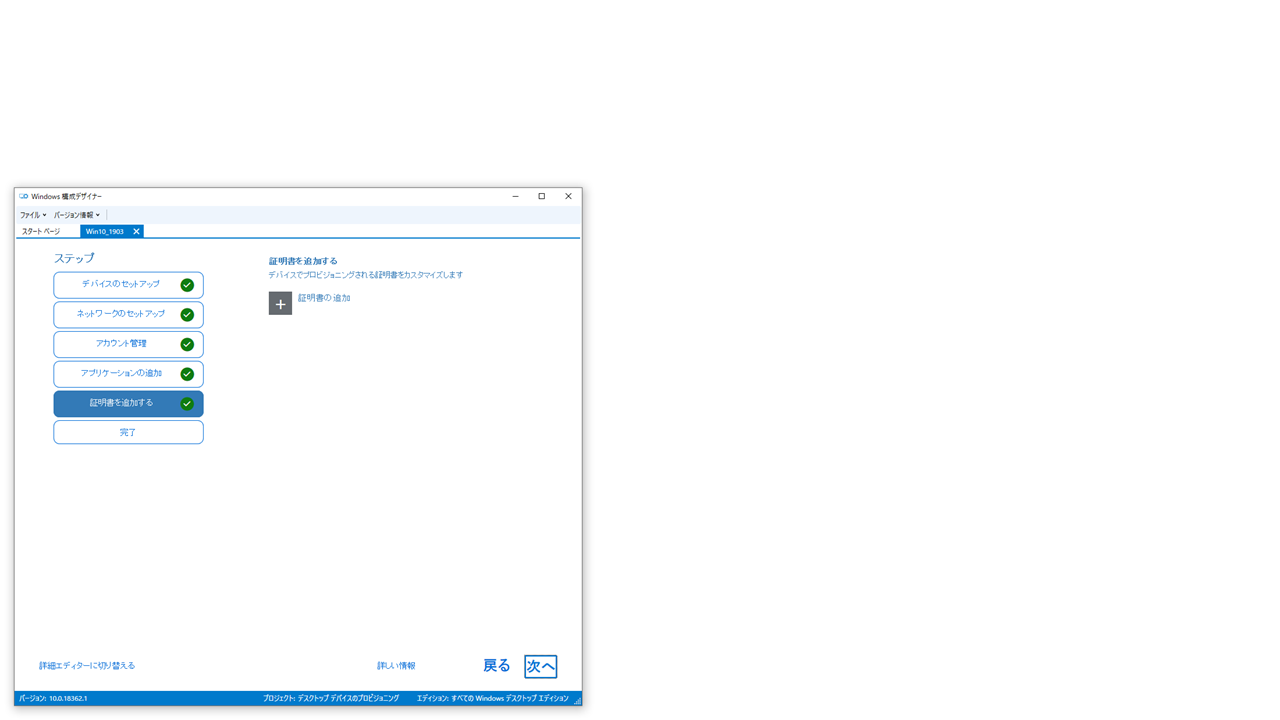
\includegraphics[width=10cm]{figures/MakeProvisioningPackage-15}
    \end{minipage}
    \begin{minipage}{0.4\textwidth}
        \textbf{「証明書の追加」}では、証明書の追加を行うことができます。
    \end{minipage}
\end{figure*}

\begin{figure*}[hp]
    \begin{minipage}{0.6\textwidth}
        \vspace{-1cm}
        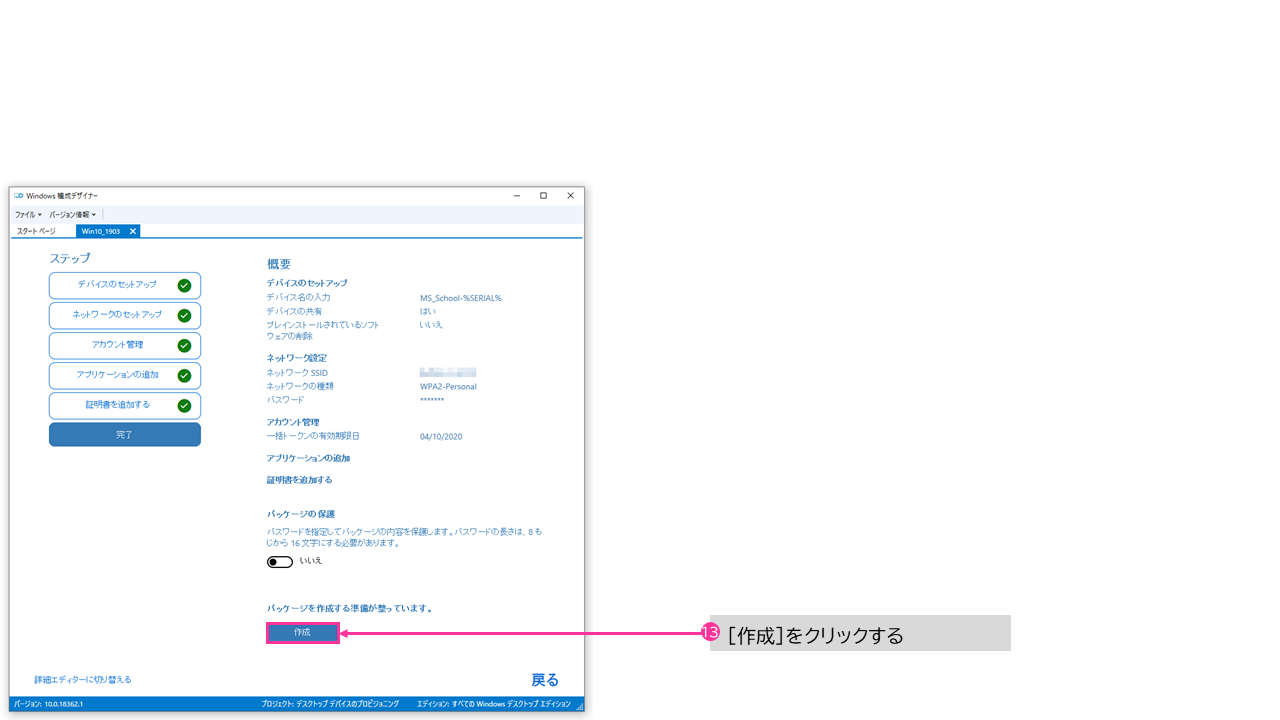
\includegraphics[width=10cm]{figures/MakeProvisioningPackage-16}
    \end{minipage}
    \begin{minipage}{0.4\textwidth}
       最後に設定した内容が表示されますので、設定内容を確認して問題ないようであれば、\textbf{【作成】}をクリックしてください。プロジェクトフォルダに拡張子がppkgとついたProvisioing Packageが作成されます。
    \end{minipage}
\end{figure*}

\begin{figure*}[hp]
    \begin{minipage}{0.6\textwidth}
        \vspace{-1cm}
        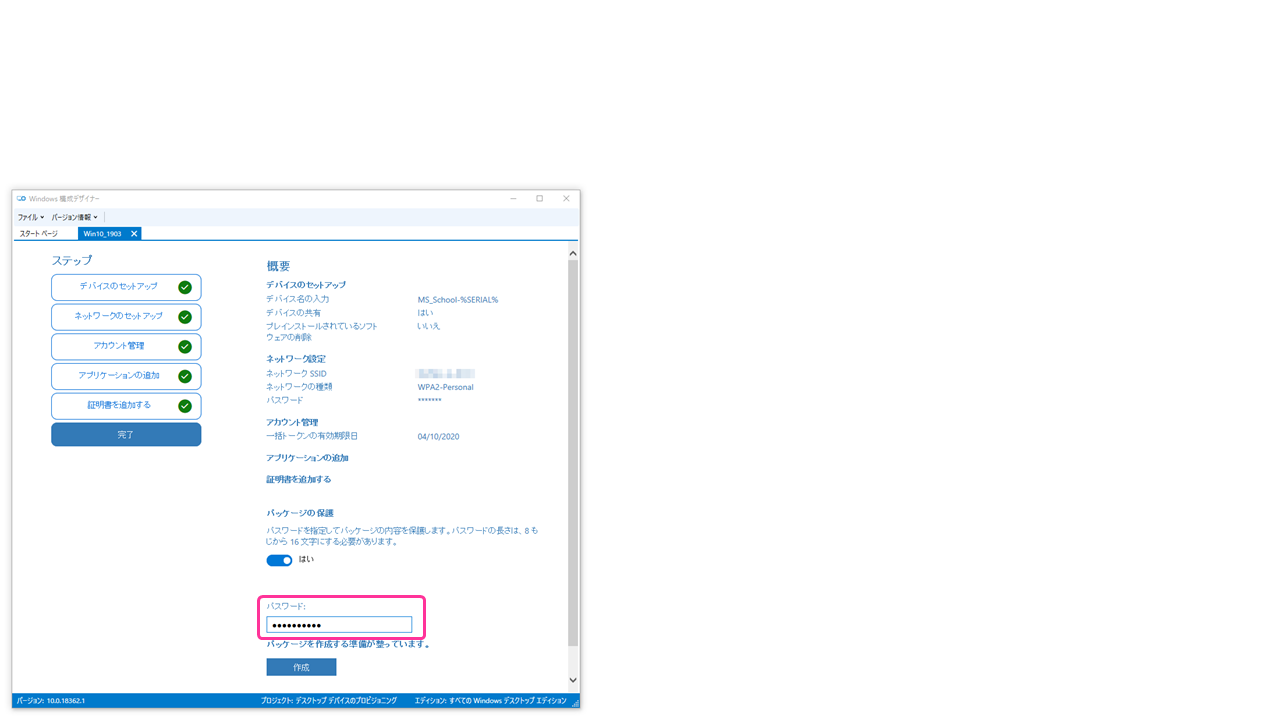
\includegraphics[width=10cm]{figures/MakeProvisioningPackage-17}
    \end{minipage}
    \begin{minipage}{0.4\textwidth}
       作成したパッケージを保護したい場合には、パスワードを設定することが可能です。パスワードを設定しますと、Provisioning Package を適用するときにパスワードの入力が求められます。
    \end{minipage}
    \vspace{8cm}
\end{figure*}


%%%%%%%%%%%%%%%%%%%%%%%%%%%%%%%%%%%%%%%%%%%%%%%%%%%%%%%%%%%%%%%%%%%%%%%%%%%%%%%%%
\begin{figure}[htbp]
    \subsection{Provisioning Package によるWindows 端末のディプロイ}
    \label{sec:ProvisioningPackageによるWindows端末のディプロイ}
\end{figure}
%%%%%%%%%%%%%%%%%%%%%%%%%%%%%%%%%%%%%%%%%%%%%%%%%%%%%%%%%%%%%%%%%%%%%%%%%%%%%%%%%

\begin{figure*}[hp]
    \begin{minipage}{0.6\textwidth}
        \vspace{-1cm}
        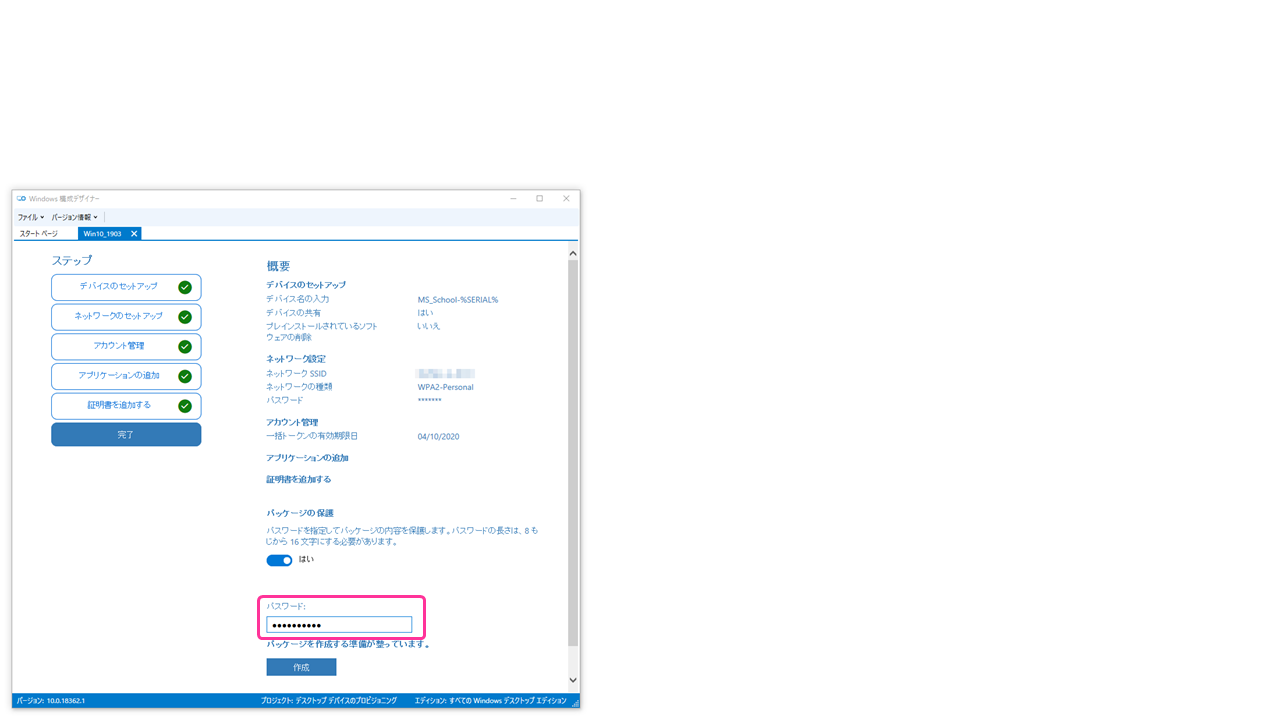
\includegraphics[width=10cm]{figures/MakeProvisioningPackage-17}
    \end{minipage}
    \begin{minipage}{0.4\textwidth}
        \label{sec:ProvisioningPackageの作成}項で作成したProvisioning Package を USBメモリにコピーします。
    \end{minipage}
\end{figure*}

\begin{figure*}[hp]
    \begin{minipage}{0.6\textwidth}
        \vspace{-1cm}
        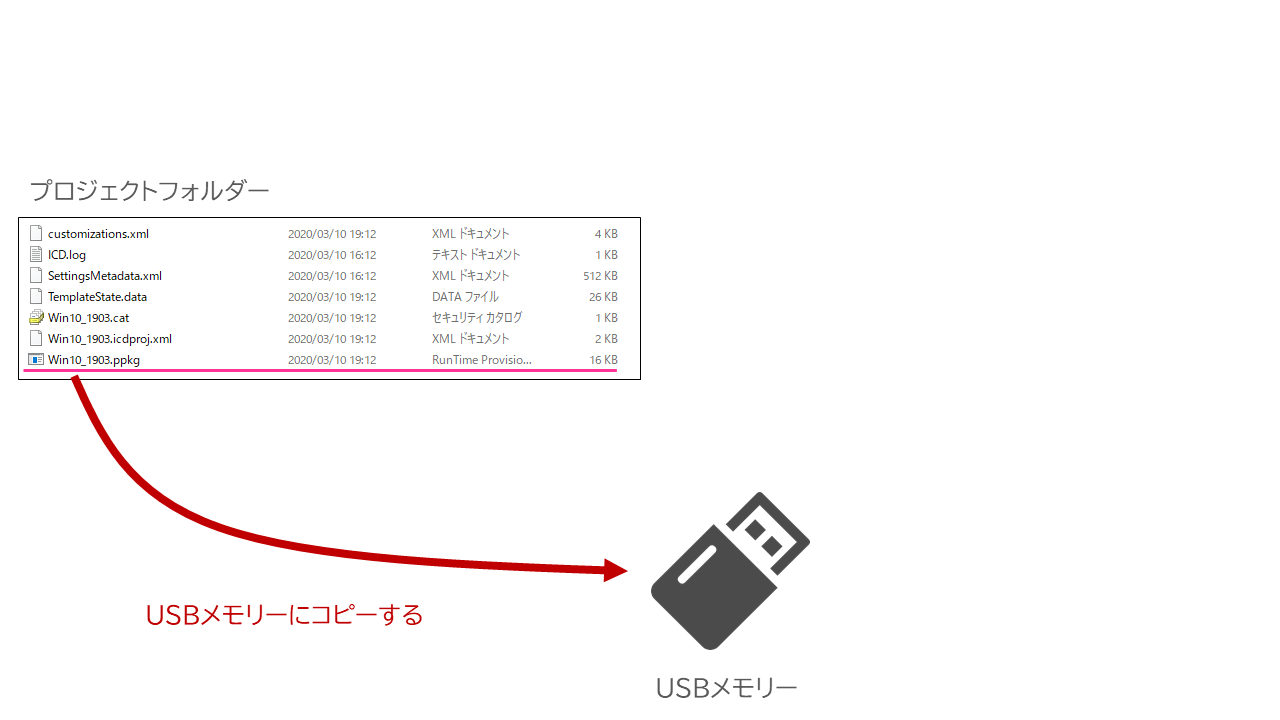
\includegraphics[width=10cm]{figures/Deploy-01.png}
    \end{minipage}
    \begin{minipage}{0.4\textwidth}
        \label{sec:ProvisioningPackageの作成}項で作成したProvisioning Package を USBメモリにコピーします。
    \end{minipage}
\end{figure*}

\begin{figure*}[hp]
    \begin{minipage}{0.6\textwidth}
        \vspace{-1cm}
        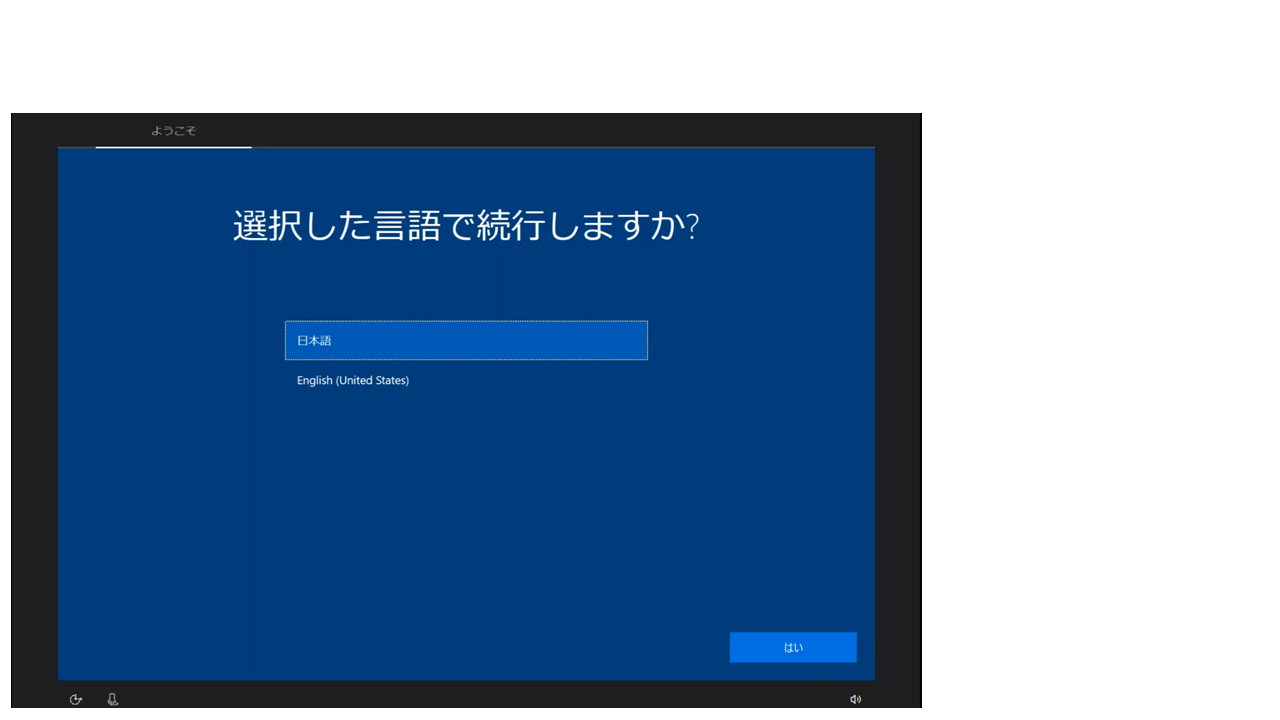
\includegraphics[width=10cm]{figures/Deploy-02.png}
    \end{minipage}
    \begin{minipage}{0.4\textwidth}
        Windows デバイスを起動し、\textbf{「選択した言語で続行しますか?」}の画面が表示されたら、Provisioing Package の入ったUSBメモリーをWindows デバイスに挿します。Provisioning Package の設定に従って、Windows デバイスは設定され、数分待つとログイン画面が表示されます。
    \end{minipage}
    \vspace{6cm}
\end{figure*}


